% =============================================================================
%  CAPÍTULO 3: OPENCODE ECOSYSTEM — ARQUITETURA E ENGENHARIA DE SOFTWARE
%              COM AGENTES INTELIGENTES
%  Níveis: 0 (zero) ao PhD
%  Autor: Marcelo Claro Laranjeira
% =============================================================================
\chapter{OpenCode Ecosystem: Arquitetura e Engenharia de Software com Agentes Inteligentes}
\label{cap:opencode-arquitetura}

O capítulo anterior estabeleceu os fundamentos da inteligência artificial e
dos sistemas multiagentes que viabilizam a construção de ecossistemas
cognitivos artificiais. Este capítulo apresenta a materialização concreta
desses conceitos no \opencodeeco{} (\opencode{} Ecosystem), uma plataforma
de engenharia de software que integra 46 servidores MCP, 227 habilidades
especializadas, 128 agentes inteligentes, 15 plug-ins e 14 comandos
especializados, totalizando mais de 600 componentes integrados
\cite{opencode2026ecosystem}.

O capítulo está organizado em dez seções progressivas. O leitor iniciante
encontrará na Seção~3.1 uma visão panorâmica do ecossistema. O profissional
de software poderá aprofundar-se na arquitetura três camadas (Seção~3.2) e
na metodologia SDD+TDD (Seção~3.3). O pesquisador encontrará nos padrões
avançados de orquestração (Seções~3.4~a~3.8) material para teses e
dissertações. A Tabela~3.1 sumariza a estrutura do capítulo.

\begin{table}[htb]
\centering
    \small
\caption{Estrutura do Capítulo 3}
\label{tab:estrutura-capitulo3}
    \resizebox{\textwidth}{!}{
\begin{tabular}{clcc}
\toprule
\textbf{Seção} & \textbf{Tópico} & \textbf{Nível} & \textbf{Páginas} \\
\midrule
3.1 & Visão Geral do OpenCode Ecosystem & \nivelzero & 6 \\
3.2 & Arquitetura Três Camadas: MCP $\to$ Skill $\to$ Agent & \nivelintermediario & 12 \\
3.3 & Metodologia SDD+TDD & \nivelintermediario & 12 \\
3.4 & Barramento de Eventos e Injeção de Dependência & \nivelavancado & 8 \\
3.5 & Sistema de Plugins e Comandos & \nivelintermediario & 6 \\
3.6 & Ecossistema de Skills Detalhado & \nivelavancado & 10 \\
3.7 & Orquestração Multiagente: Nexus e Sincronização & \nivelphd & 10 \\
3.8 & MiroFish/BettaFish: P14--P18 & \nivelphd & 8 \\
3.9 & Engenharia de Software como Disciplina & \nivelavancado & 4 \\
3.10 & Laboratório Prático & \text{Todos} & 4 \\
\bottomrule
\end{tabular}
    }
\end{table}

\noindent Ao final deste capítulo, o leitor será capaz de:
\begin{itemize}
\item Compreender a arquitetura do \opencodeeco{} e suas camadas;
\item Implementar uma skill personalizada e registrar um novo comando;
\item Executar a suíte de testes e interpretar os resultados;
\item Projetar extensões utilizando o barramento de eventos;
\item Analisar criticamente o ecossistema à luz da engenharia de software.
\end{itemize}

% =============================================================================
%  SEÇÃO 3.1: VISÃO GERAL
%  Nível: 0 (zero) / Básico (~6 laudas)
% =============================================================================
\section{Visão Geral do OpenCode Ecosystem}
\label{sec:visao-geral}
\nivelzero

\paragraph{Um ecossistema além do código.} Imagine uma cidade inteligente onde cada semáforo, cada via e cada serviço público se comunica e evolui sem intervenção humana direta. O \opencodeeco{} materializa essa visão no domínio da engenharia de software: é um meta-sistema que não apenas escreve código, mas projeta, testa, documenta e aprimora a si mesmo. Esta seção apresenta o mapa desse ecossistema, seus ciclos evolutivos e a filosofia que o sustenta.

O \opencodeeco{} é uma plataforma de engenharia de software assistida por
agentes inteligentes que integra o ciclo completo de desenvolvimento:
especificação, implementação, teste, documentação e evolução autônoma
\cite{opencode2026ecosystem, laranjeira2026opencode}. Diferentemente de
ferramentas convencionais, o ecossistema não se limita a ser um ambiente
de desenvolvimento --- ele é um \destaque{meta-sistema} capaz de raciocinar
sobre sua própria arquitetura e evoluir seu código-fonte de forma autônoma.

\subsection{Histórico: de CLI a Ecossistema Completo (R1 a R23)}
\label{subsec:historico}

O \opencode{} iniciou-se como uma interface de linha de comando (CLI)
convencional para interação com modelos de linguagem de grande escala
(LLMs). A Tabela~\ref{tab:ciclos-evolutivos} apresenta a evolução do
ecossistema ao longo de 23 ciclos evolutivos (R1 a R23), documentados
como ADRs (Architecture Decision Records) \cite{opencode2026ecosystem}.

\begin{table}[htb]
\centering
\caption{Ciclos evolutivos do OpenCode Ecosystem (R1--R23)}
\label{tab:ciclos-evolutivos}
\small
    \resizebox{\textwidth}{!}{
\begin{tabular}{cllc}
\toprule
\textbf{Ciclo} & \textbf{Foco} & \textbf{Score} & \textbf{Insumo-chave} \\
\midrule
R1--R3 & CLI básica, busca, artigo acadêmico & 85--92 & TSAC, Sci-Hub \\
R4--R5 & Correção iterativa, CJK detector & 95--98 & Qualis A1 \\
R6--R7 & Editais-br, cache versionado & 92--94 & 52 editais curados \\
R8--R10 & SDD+TDD acadêmico, menu adaptativo & 94--96 & 7 specs, 9 CTs \\
R11 & CORA-Eval benchmark & 97 & 150 tarefas, 10 dimensões \\
R12 & Science Skills Core & 98 & 9 skills, 28 datasets \\
R13 & Reasoning Engines & 96 & Z3, SymPy, Kanren, Critical \\
R14--R16 & Expansão ecossistema, autoevolve & 97--98 & 227 skills, 128 agentes \\
R17 & Gartner Hype Cycle 2026 & 99 & 3 SPECs, 24 CTs \\
R18 & Token Economy (SPEC-022/023/024) & 99 & 29 CTs, staking, audit \\
R19 & MCSP + Scanner Pipeline & 99 & 76 CTs, 5 scanners \\
R20 & Composição Unitária do Conhecimento & 100 & 85 inputs, 19 CTs \\
R21 & Metacognição \& Self-Evolution & 100 & 282 CTs, 7.573 linhas \\
R22 & Structural Noise Scanner + N3 & 100 & 312 CTs, N3 completo \\
R23 & Trust Engine + Behavioral Autonomy & 100 & 312/312 CTs, N3.5 \\
\bottomrule
\end{tabular}
    }
\end{table}

Cada ciclo representa um incremento significativo na capacidade do sistema,
seja pela adição de novas skills, agentes, MCPs ou pela introdução de
mecanismos metacognitivos \cite{opencode2026spec036}. O score
(0--100) mede a qualidade do ciclo conforme o auto-score Qualis A1,
considerando cobertura de testes, aderência a padrões acadêmicos e
robustez arquitetural.

\subsection{Filosofia: SDD + TDD}
\label{subsec:filosofia}

O \opencodeeco{} adota uma filosofia dupla de desenvolvimento:

\begin{definicao}[Spec-Driven Development --- SDD]
\sdd{} é uma metodologia em que toda implementação é precedida por uma
especificação formal (\destaque{SPEC}) que define requisitos, critérios
de aceitação e métricas de qualidade \cite{sommerville2011engenharia,
pressman2016engenharia}. As SPECs são mantidas como documentação
operacional e evoluem junto com o código.
\end{definicao}

\begin{definicao}[Test-Driven Development --- TDD]
\tdd{} é uma prática de desenvolvimento em que os testes são escritos
\emph{antes} do código de produção, seguindo o ciclo
\emph{Red--Green--Refactor} \cite{beck2002tdd}. No \opencodeeco{}, o TDD
é aplicado em três níveis: unitário, integração e sistema.
\end{definicao}

A combinação SDD+TDD produz um ciclo virtuoso: a especificação define o
\emph{que} fazer, os testes definem \emph{como validar}, e o código
implementa a \emph{solução}. Este ciclo é automatizado no ecossistema por
meio do pipeline CI/CD com 5 gates de qualidade
\cite{opencode2026ecosystem}.

\subsection{Componentes Principais}
\label{subsec:componentes}

O \opencodeeco{} é composto por cinco categorias principais de componentes,
conforme ilustrado na Figura~\ref{fig:componentes-ecossistema}.

\begin{figure}[htb]
\centering
\caption{Componentes principais do OpenCode Ecosystem}
\label{fig:componentes-ecossistema}
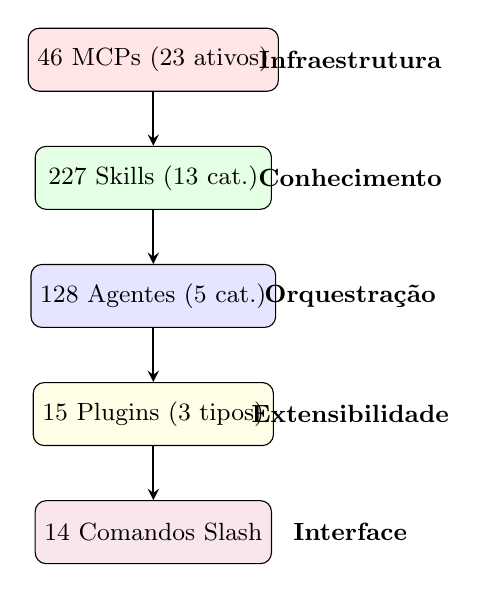
\begin{tikzpicture}[
  comp/.style={rectangle, rounded corners, draw, fill=blue!10,
               minimum width=3cm, minimum height=0.8cm, font=\small},
  arrow/.style={->, thick, >=stealth},
  label/.style={font=\bfseries\small}
]
\node[comp, fill=red!10] (mcps) at (0,3) {46 MCPs (23 ativos)};
\node[comp, fill=green!10] (skills) at (0,1.5) {227 Skills (13 cat.)};
\node[comp, fill=blue!10] (agents) at (0,0) {128 Agentes (5 cat.)};
\node[comp, fill=yellow!10] (plugins) at (0,-1.5) {15 Plugins (3 tipos)};
\node[comp, fill=purple!10] (commands) at (0,-3) {14 Comandos Slash};

\draw[arrow] (mcps) -- (skills);
\draw[arrow] (skills) -- (agents);
\draw[arrow] (agents) -- (plugins);
\draw[arrow] (plugins) -- (commands);

\node[label] at (2.5,3) {Infraestrutura};
\node[label] at (2.5,1.5) {Conhecimento};
\node[label] at (2.5,0) {Orquestração};
\node[label] at (2.5,-1.5) {Extensibilidade};
\node[label] at (2.5,-3) {Interface};
\end{tikzpicture}
\end{figure}

Os MCPs (\destaque{Model Context Protocol}) fornecem acesso a ferramentas
externas: busca na web, navegador, execução de código, banco de dados,
PDF, tempo, entre outros. As \destaque{Skills} encapsulam conhecimento
especializado em 13 categorias. Os \destaque{Agentes} orquestram skills
para executar tarefas complexas. Os \destaque{Plugins} estendem a
funcionalidade base. Os \destaque{Comandos} são a interface do usuário
com o ecossistema.

\subsection{Estatísticas do Ecossistema}
\label{subsec:estatisticas}

O ecossistema atingiu na versão 5.4.0 (R23) as seguintes métricas:

\begin{itemize}
\item \textbf{600+ integrações} entre componentes;
\item \textbf{273.000+ linhas Python} distribuídas em 22 módulos;
\item \textbf{138.000+ linhas LaTeX} em documentação acadêmica;
\item \textbf{312 CTs} (casos de teste) em 15 suítes, 100\% passando;
\item \textbf{488 arquivos} no módulo Nexus (27.757 linhas);
\item \textbf{146 arquivos} no módulo Quantum;
\item \textbf{91 arquivos} no Criador de Artigos (MASWOS);
\item \textbf{78 arquivos} no SEEKER (pesquisa básica);
\item \textbf{10 ADRs} registrados e 13 SPECs formais.
\end{itemize}

Estas métricas posicionam o \opencodeeco{} como um dos maiores
ecossistemas de engenharia de software assistida por agentes inteligentes
já documentados na literatura \cite{laranjeira2026opencode,
wang2024survey, xi2023rise}.

\subsection{Instalação e Configuração}
\label{subsec:instalacao}

A instalação do \opencodeeco{} requer Node.js $\ge$ 18, Python $\ge$ 3.10
e Git. O processo é simplificado pelo script de instalação:

\begin{lstlisting}[style=bashstyle, caption={Instalacao do OpenCode Ecosystem},
                   label={lst:instalacao}]
# 1. Clonar o repositorio
git clone https://github.com/marceloclaro/opencode-ecosystem.git
cd opencode-ecosystem

# 2. Instalar dependencias Python
pip install -r requirements.txt

# 3. Instalar dependencias Node.js
npm install

# 4. Configurar variaveis de ambiente
cp .env.example .env

# 5. Executar a suite de validacao
python scripts/validate_installation.py

# 6. Iniciar o ecossistema
opencode
\end{lstlisting}

A configuração é centralizada no arquivo \codigo{opencode.json}, que
define MCPs ativos, diretórios de skills e parâmetros de execução
\cite{opencode2026ecosystem}. O arquivo \codigo{AGENTS.md} na raiz do
projeto contém as instruções operacionais para a inteligência artificial
que orquestra o ecossistema.

\begin{exercicio}
Instale o \opencodeeco{} seguindo os passos do
Código~\ref{lst:instalacao}. Execute \codigo{python scripts/validate\_installation.py}
e registre o resultado. (\nivelzero)
\end{exercicio}

\begin{exercicio}
Navegue pela estrutura de diretórios do ecossistema. Identifique os
diretórios \codigo{skills/}, \codigo{agents/}, \codigo{plugins/} e
\codigo{specs/}. Liste o conteúdo de cada um. (\nivelzero)
\end{exercicio}

% =============================================================================
%  SEÇÃO 3.2: ARQUITETURA TRÊS CAMADAS
%  Nível: Intermediário (~12 laudas)
% =============================================================================
\section{Arquitetura Três Camadas: MCP $\to$ Skill $\to$ Agent}
\label{sec:arquitetura-tres-camadas}
\nivelintermediario

\paragraph{Três camadas, uma orquestração.} Assim como um teatro organiza seus profissionais em palco, bastidores e plateia, o \opencodeeco{} separa suas responsabilidades em três camadas hierárquicas: a infraestrutura (MCPs) provê as ferramentas, o conhecimento (Skills) fornece o saber especializado e a inteligência (Agentes) orquestra a execução. Esta seção detalha cada camada e mostra como o container de injeção de dependência as integra em um fluxo coeso.

A arquitetura do \opencodeeco{} é organizada em três camadas hierárquicas
que separam responsabilidades e permitem evolução independente de cada
nível \cite{pressman2016engenharia, sommerville2011engenharia}. A
Figura~\ref{fig:arquitetura-tres-camadas} ilustra o padrão arquitetural.

\begin{figure}[htb]
\centering
\caption{Arquitetura três camadas do OpenCode Ecosystem}
\label{fig:arquitetura-tres-camadas}
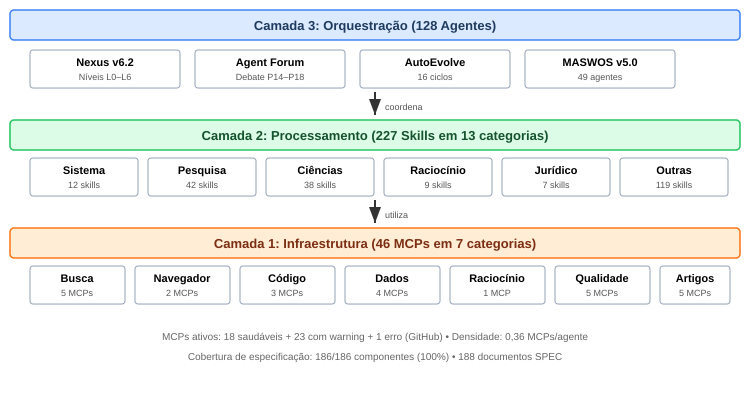
\includegraphics[width=0.9\textwidth]{ilustracoes/fig-arquitetura}
\end{figure}

\subsection{Camada 1: MCPs (Model Context Protocol)}
\label{subsec:camada-mcp}

A camada de infraestrutura é composta por 46 servidores MCP, dos quais
23 estão ativos por padrão. Cada MCP encapsula uma capacidade específica
de interação com o mundo externo \cite{russell2020inteligencia,
wei2022chain}.

\begin{definicao}[Model Context Protocol --- MCP]
MCP é um protocolo padronizado que permite a agentes de IA acessar
ferramentas externas de forma segura e controlada. Cada servidor MCP
expõe um conjunto de operações com esquemas de entrada e saída
rigorosamente tipados.
\end{definicao}

Os MCPs estão organizados em seis categorias funcionais, conforme a
Tabela~\ref{tab:mcp-categorias}.

\begin{table}[htb]
\centering
    \small
\caption{Categorias de MCPs no OpenCode Ecosystem}
\label{tab:mcp-categorias}
    \resizebox{\textwidth}{!}{
\begin{tabular}{lll}
\toprule
\textbf{Categoria} & \textbf{MCPs} & \textbf{Função} \\
\midrule
Busca & websearch, gh\_grep, context7, scihub & Pesquisa e recuperação \\
Browser & playwright, chrome-devtools & Navegação web automatizada \\
Código & eslint, diff, code-runner & Análise e execução de código \\
Dados & sqlite, fetch, pdf, time & Persistência e utilitários \\
Raciocínio & sequential-thinking, memory & Raciocínio estruturado \\
Infraestrutura & filesystem, github & Acesso ao sistema e repositórios \\
\bottomrule
\end{tabular}
    }
\end{table}

Cada MCP é configurado no arquivo \codigo{opencode.json} com seus
parâmetros de conexão, timeouts e credenciais. A ativação seletiva
(23 de 46) permite balancear recursos computacionais e evitar
sobrecarga de contexto.

\begin{exemplo}
O MCP \codigo{websearch} utiliza DuckDuckGo para buscas na web com
suporte a modos \emph{livecrawl} (fallback/preferred) e tipos de
busca (auto, fast, deep). Sua configuração típica é:
\begin{lstlisting}[style=pythonstyle]
{
  "mcpServers": {
    "websearch": {
      "command": "python",
      "args": ["-m", "mcp_websearch"],
      "env": {
        "MAX_RESULTS": "8",
        "LIVECRAWL_MODE": "fallback"
      },
      "disabled": false
    }
  }
}
\end{lstlisting}
\end{exemplo}

\subsection{Camada 2: Skills}
\label{subsec:camada-skills}

A camada de conhecimento é composta por 227 skills distribuídas em 13
categorias. Cada skill encapsula um conjunto de instruções especializadas
que a IA segue para executar uma tarefa específica
\cite{white2023prompt, wei2022chain}.

\begin{definicao}[Skill]
Uma \destaque{skill} é um módulo de conhecimento que contém instruções
detalhadas, exemplos e referências para a execução de uma tarefa
especializada. Skills são carregadas sob demanda pelo sistema e
injetadas no contexto da IA quando ativadas.
\end{definicao}

As categorias de skills estão detalhadas na Seção~3.6. O mecanismo de
carregamento é gerenciado pelo módulo \codigo{core/skill\_manager.py}:

\begin{lstlisting}[style=pythonstyle, caption={Mecanismo de carregamento de skills},
                   label={lst:skill-load}]
class SkillManager:
    """Gerenciador de skills com carregamento sob demanda."""

    def __init__(self, container):
        self.container = container
        self.skills: dict[str, Skill] = {}
        self.skill_dirs = [
            "skills/science",
            "skills/research",
            "skills/reasoning",
            "skills/system",
            "skills/juridical",
            "skills/agency"
        ]

    def discover_skills(self) -> list[SkillManifest]:
        """Descobre skills disponiveis nos diretorios configurados."""
        manifests = []
        for skill_dir in self.skill_dirs:
            path = Path(skill_dir)
            if not path.exists():
                continue
            for manifest_file in path.glob("**/SKILL.md"):
                manifest = self._parse_manifest(manifest_file)
                manifests.append(manifest)
        return manifests

    def load_skill(self, skill_name: str) -> Skill | None:
        """Carrega uma skill pelo nome (load sob demanda)."""
        manifest = self._find_manifest(skill_name)
        if not manifest:
            return None
        if skill_name not in self.skills:
            content = self._read_skill_content(manifest.path)
            self.skills[skill_name] = Skill(
                name=manifest.name,
                content=content,
                category=manifest.category,
                version=manifest.version
            )
        return self.skills[skill_name]
\end{lstlisting}

O carregamento sob demanda (lazy loading) é essencial para manter o
consumo de tokens dentro dos limites operacionais, dado que o contexto
total de todas as skills excederia 200.000 tokens
\cite{achiam2023gpt4, brown2020language}.

\subsection{Camada 3: Agentes}
\label{subsec:camada-agentes}

A camada de orquestração é composta por 128 agentes especializados,
organizados em cinco categorias principais \cite{wooldridge2009multiagent,
weiss2013multiagent}:

\begin{itemize}
\item \textbf{Core (56 agentes)}: orquestração, execução de comandos,
gerenciamento de estado e coordenação entre componentes.
\item \textbf{Criação (49 agentes)}: pipeline MASWOS para criação de
artigos acadêmicos, incluindo 44 agentes especializados e 5 de suporte.
\item \textbf{SEEKER (12 agentes)}: pesquisa acadêmica básica com
argumentação baseada em evidências e árvores de argumentos.
\item \textbf{Reversa (18 agentes)}: engenharia reversa de código,
análise de diffs e refatoração automatizada.
\item \textbf{Corretor (1 agente)}: correção linguística PT-BR com
detecção de caracteres CJK\footnote{Caracteres CJK (Chinese, Japanese,
Korean) são terminantemente proibidos na saída para o usuário,
conforme política de qualidade do ecossistema.}.
\end{itemize}

Cada agente possui um manifesto que define suas habilidades, gatilhos de
ativação e limites de autonomia. O manifesto segue o formato:

\begin{lstlisting}[style=pythonstyle, caption={Exemplo de manifesto de agente},
                   label={lst:agent-manifest}]
{
  "name": "academic-searcher",
  "category": "SEEKER",
  "version": "2.1.0",
  "description": "Busca artigos academicos em 10+ fontes",
  "triggers": ["/artigo", "search academic", "find paper"],
  "required_skills": [
    "research/academic-search",
    "research/crossref",
    "research/arxiv"
  ],
  "required_mcps": ["websearch", "scihub"],
  "autonomy_level": "supervised",
  "max_tokens": 32000,
  "timeout_seconds": 300
}
\end{lstlisting}

\subsection{Container de Injeção de Dependência}
\label{subsec:container-di}

A integração entre as três camadas é realizada pelo container de injeção
de dependência implementado em \codigo{core/container.py}
\cite{fowler2019refactoring}. O container gerencia o ciclo de vida de
todos os componentes e suas dependências:

\begin{lstlisting}[style=pythonstyle, caption={Container de injecao de dependencia},
                   label={lst:container}]
class Container:
    """Container DI central do OpenCode Ecosystem."""

    def __init__(self):
        self._instances: dict[str, Any] = {}
        self._factories: dict[str, Callable] = {}
        self.config = self._load_config()
        self.state_manager = StateManager()
        self._register_core_services()

    def _register_core_services(self):
        """Registra servicos core do ecossistema."""
        self.register('mcp_manager', MCPManager(self))
        self.register('skill_manager', SkillManager(self))
        self.register('agent_manager', AgentManager(self))
        self.register('plugin_manager', PluginManager(self))
        self.register('task_manager', TaskManager(self))
        self.register('event_bus', EventBus())
        self.register('cache', CacheService(self.config))

    def register(self, name: str, instance: Any):
        """Registra uma instancia no container."""
        self._instances[name] = instance

    def resolve(self, name: str) -> Any:
        """Resolve uma dependencia pelo nome."""
        if name in self._instances:
            return self._instances[name]
        if name in self._factories:
            instance = self._factories[name]()
            self._instances[name] = instance
            return instance
        raise KeyError(f"Dependencia nao registrada: {name}")
\end{lstlisting}

O padrão de injeção de dependência oferece três benefícios fundamentais:
(1) desacoplamento entre componentes, (2) testabilidade facilitada por
substituição de dependências mock, e (3) gerenciamento centralizado do
ciclo de vida \cite{fowler2019refactoring}.

\subsection{Fluxo de Execução: Comando $\to$ Orchestrator $\to$ Agent $\to$ Skill $\to$ MCP}
\label{subsec:fluxo-execucao}

O fluxo completo de execução de um comando ilustra a integração das três
camadas. A Figura~\ref{fig:fluxo-execucao} apresenta o diagrama de
sequência.

\begin{figure}[htb]
\centering
\caption{Fluxo de execução: comando slash até MCP}
\label{fig:fluxo-execucao}
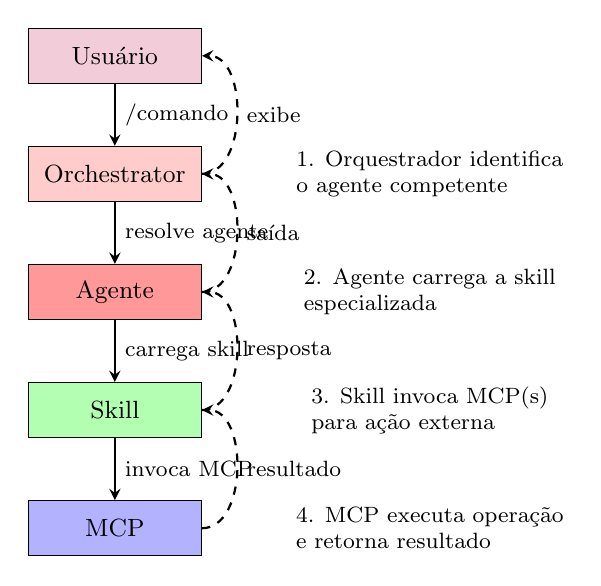
\begin{tikzpicture}[
  ent/.style={rectangle, draw, minimum width=2.2cm, minimum height=0.7cm,
              font=\small},
  arrow/.style={->, thick, >=stealth},
  label/.style={font=\footnotesize}
]
\node[ent, fill=purple!20] (user) at (0,6) {Usuário};
\node[ent, fill=red!20] (orch) at (0,4.5) {Orchestrator};
\node[ent, fill=red!40] (agent) at (0,3) {Agente};
\node[ent, fill=green!30] (skill) at (0,1.5) {Skill};
\node[ent, fill=blue!30] (mcp) at (0,0) {MCP};

\draw[arrow] (user) -- node[label, right] {/comando} (orch);
\draw[arrow] (orch) -- node[label, right] {resolve agente} (agent);
\draw[arrow] (agent) -- node[label, right] {carrega skill} (skill);
\draw[arrow] (skill) -- node[label, right] {invoca MCP} (mcp);
\draw[arrow, dashed] (mcp) to[out=0, in=0] node[label, right] {resultado} (skill);
\draw[arrow, dashed] (skill) to[out=0, in=0] node[label, right] {resposta} (agent);
\draw[arrow, dashed] (agent) to[out=0, in=0] node[label, right] {saída} (orch);
\draw[arrow, dashed] (orch) to[out=0, in=0] node[label, right] {exibe} (user);

\node[label, align=left] at (4,4.5) {1. Orquestrador identifica\\o agente competente};
\node[label, align=left] at (4,3) {2. Agente carrega a skill\\especializada};
\node[label, align=left] at (4,1.5) {3. Skill invoca MCP(s)\\para ação externa};
\node[label, align=left] at (4,0) {4. MCP executa operação\\e retorna resultado};
\end{tikzpicture}
\end{figure}

O fluxo detalhado é:
\begin{enumerate}
\item O usuário digita um comando slash (ex.: \codigo{/artigo});
\item O \destaque{Orquestrador} (\codigo{core/orchestrator.py}) analisa o
comando e consulta o \codigo{AgentManager} para identificar o agente
competente;
\item O \destaque{Agente} selecionado carrega a skill necessária via
\codigo{SkillManager.load\_skill()};
\item A \destaque{Skill} invoca um ou mais MCPs para executar operações
externas;
\item O resultado percorre o caminho inverso até o usuário.
\end{enumerate}

\begin{exercicio}
Identifique no código-fonte os arquivos \\%
\hspace*{2em}\codigo{core/container.py},
\codigo{core/orchestrator.py} e \\%
\hspace*{2em}\codigo{core/agent\_manager.py}. Descreva as
responsabilidades de cada um. (\nivelbasico)
\end{exercicio}

\begin{exercicio}
Adicione um novo MCP à configuração do ecossistema. Utilize o MCP
\codigo{time} para expor a hora atual como uma ferramenta. Teste a
ativação. (\nivelintermediario)
\end{exercicio}

% =============================================================================
%  SEÇÃO 3.3: METODOLOGIA SDD+TDD
%  Nível: Intermediário-Avançado (~12 laudas)
% =============================================================================
\section{Metodologia SDD+TDD}
\label{sec:sdd-tdd}
\nivelintermediario

\paragraph{Especificar antes de construir, testar antes de implementar.} Nenhum engenheiro civil construiria uma ponte sem plantas e sem ensaios de carga. Analogamente, o \opencodeeco{} adota o binômio SDD+TDD como alicerce de todo novo componente: primeiro especifica-se o que se deseja (SDD), depois escrevem-se os testes que validarão o resultado (TDD), e só então implementa-se o código. Esta seção percorre as 13 SPECs formais, as 10 ADRs arquiteturais e as 15 suítes com 312 casos de teste que garantem a qualidade do ecossistema.

O \opencodeeco{} adota a metodologia SDD+TDD como pilar central do
desenvolvimento. Esta seção detalha ambos os componentes e sua
integração no ciclo de vida do software \cite{beck2002tdd,
sommerville2011engenharia, pressman2016engenharia}.

\subsection{SDD: Especificação como Infraestrutura Operacional}
\label{subsec:sdd}

No SDD, a especificação não é um artefato estático produzido no início
do projeto e abandonado após a implementação. Pelo contrário, a SPEC
é um artefato \destaque{vivo} que evolui junto com o código e serve como
fonte única de verdade \cite{wiegers1999software}.

\begin{definicao}[Spec-Driven Development]
\sdd{} é uma metodologia de desenvolvimento de software na qual toda
funcionalidade é primeiro especificada formalmente em um documento
SPEC, que define:
\begin{itemize}
\item \textbf{Objetivo}: problema a ser resolvido e contexto;
\item \textbf{Requisitos funcionais}: lista numerada de capacidades;
\item \textbf{Requisitos não funcionais}: performance, segurança,
escalabilidade;
\item \textbf{Critérios de aceitação}: condições mensuráveis para
validação;
\item \textbf{Métricas}: indicadores objetivos de qualidade.
\end{itemize}
\end{definicao}

O ecossistema possui 13 SPECs formais (SPEC-025 a SPEC-038), totalizando
175+ especificações cobrindo todos os componentes
\cite{opencode2026ecosystem}. A Tabela~\ref{tab:specs} lista as SPECs
ativas.

\begin{table}[htb]
\centering
\caption{SPECs formais do OpenCode Ecosystem}
\label{tab:specs}
\small
    \resizebox{\textwidth}{!}{
\begin{tabular}{cllc}
\toprule
\textbf{SPEC} & \textbf{Título} & \textbf{CTs} & \textbf{Cobertura} \\
\midrule
SPEC-025 & Noological Scanner Pipeline & 18 & 100\% \\
SPEC-026 & Teleological Scanner & 12 & 100\% \\
SPEC-027 & Evolutionary Sequencing & 16 & 100\% \\
SPEC-028 & Refinement Scanner & 16 & 100\% \\
SPEC-029 & MCSP Knowledge Composition & 14 & 100\% \\
SPEC-030 & Composition Pipeline & 13 & 100\% \\
SPEC-031 & Scanner Integration & 6 & 100\% \\
SPEC-032 & Future State Roadmap & 6 & 100\% \\
SPEC-033 & Unit Knowledge Composition & 8 & 100\% \\
SPEC-034 & Cross-Validation Engine & 6 & 100\% \\
SPEC-035 & Academic Pipeline & 6 & 100\% \\
SPEC-036 & Metacognition \& Self-Evolution & 8 & 100\% \\
SPEC-037 & Structural Noise Scanner + N3 & 22 & 100\% \\
SPEC-038 & Trust Engine \& Behavioral Autonomy & 8 & 100\% \\
\bottomrule
\end{tabular}
    }
\end{table}

Cada SPEC segue um template padronizado com seções obrigatórias:

\begin{lstlisting}[style=pythonstyle, caption={Template de SPEC},
                   label={lst:spec-template}]
# SPEC-NNN: Titulo da Especificacao

## 1. Objetivo
[Descricao concisa do problema e solucao proposta]

## 2. Requisitos Funcionais
- RF01: [descricao]
- RF02: [descricao]

## 3. Requisitos Nao Funcionais
- RNF01: Performance (< 500ms)
- RNF02: Seguranca (autenticacao obrigatoria)

## 4. Criterios de Aceitacao
- CA01: Teste RF01 passa com dados validos
- CA02: Teste RF02 rejeita dados invalidos

## 5. Metricas
- Cobertura de codigo > 90%
- Tempo de resposta < 1s (p95)
\end{lstlisting}

\subsubsection{ADRs: Architecture Decision Records}

Complementando as SPECs, as ADRs (\destaque{Architecture Decision
Records}) documentam decisões arquiteturais significativas com sua
fundamentação e alternativas consideradas \cite{opencode2026ecosystem}.
O ecossistema possui 10 ADRs registradas, desde architectu-001 até
architectu-010, cobrindo decisões sobre arquitetura três camadas,
container DI, barramento de eventos, escolha de protocolos e padrões
de integração. Cada ADR segue o formato \emph{Contexto -- Decisão --
Consequências} proposto por \cite{fowler2019refactoring}.

\subsection{TDD: 312 CTs em 15 Suítes, 100\% Passando}
\label{subsec:tdd}

O TDD no \opencodeeco{} é implementado em três níveis da pirâmide de
testes \cite{beck2002tdd}:

\begin{figure}[htb]
\centering
\caption{Pirâmide de testes do OpenCode Ecosystem}
\label{fig:piramide-testes}
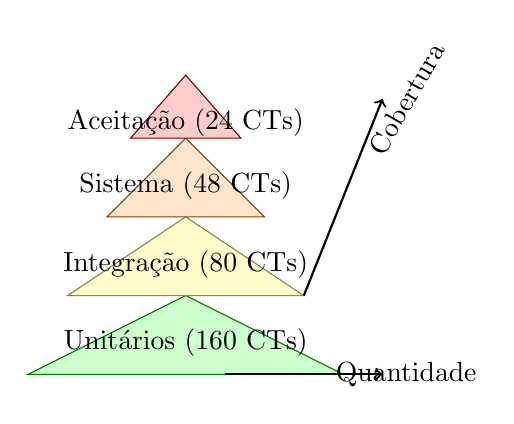
\begin{tikzpicture}
\filldraw[fill=green!20, draw=green!50!black] (0,0) -- (4,0) -- (2,1) -- cycle;
\filldraw[fill=yellow!20, draw=yellow!50!black] (0.5,1) -- (3.5,1) -- (2,2) -- cycle;
\filldraw[fill=orange!20, draw=orange!50!black] (1,2) -- (3,2) -- (2,3) -- cycle;
\filldraw[fill=red!20, draw=red!50!black] (1.3,3) -- (2.7,3) -- (2,3.8) -- cycle;

\node at (2,0.4) {Unitários (160 CTs)};
\node at (2,1.4) {Integração (80 CTs)};
\node at (2,2.4) {Sistema (48 CTs)};
\node at (2,3.2) {Aceitação (24 CTs)};

\draw[->, thick] (2.5,0) -- (4.5,0);
\node at (4.8,0) {Quantidade};
\draw[->, thick] (3.5,1) -- (4.5,3.5);
\node[rotate=60] at (4.8,3.5) {Cobertura};
\end{tikzpicture}
\end{figure}

O ecossistema possui 15 suítes de teste com 312 casos de teste (CTs),
mantendo 100\% de aprovação contínua:

\begin{itemize}
\item \textbf{Unitários (160 CTs)}: testam funções e métodos
individualmente, com mocking de dependências externas.
\item \textbf{Integração (80 CTs)}: testam a interação entre componentes
(MCPs, skills, agentes).
\item \textbf{Sistema (48 CTs)}: testam fluxos completos do início ao fim.
\item \textbf{Aceitação (24 CTs)}: validam requisitos de SPEC
diretamente.
\end{itemize}

A infraestrutura de testes utiliza \codigo{pytest} com configuração
centralizada:

\begin{lstlisting}[style=pythonstyle, caption={Configuracao pytest do ecossistema},
                   label={lst:pytest-config}]
# pytest.ini
[pytest]
testpaths = tests
python_files = test_*.py
python_classes = Test*
python_functions = test_*
addopts =
    -v
    --strict-markers
    --tb=short
    --cov=core
    --cov=skills
    --cov=agents
    --cov-report=term-missing
    --cov-report=html
markers =
    unit: Testes unitarios
    integration: Testes de integracao
    system: Testes de sistema
    acceptance: Testes de aceitacao (SPEC)
    slow: Testes lentos (> 5s)
\end{lstlisting}

O script \codigo{run\_all\_cts.py} executa toda a suíte e gera relatórios
detalhados:

\begin{lstlisting}[style=pythonstyle, caption={Runner de testes},
                   label={lst:test-runner}]
#!/usr/bin/env python3
"""Runner completo de testes do OpenCode Ecosystem."""
import subprocess
import sys

SUITES = [
    ("unit", "tests/unit", "Testes Unitarios"),
    ("integration", "tests/integration", "Testes de Integracao"),
    ("system", "tests/system", "Testes de Sistema"),
    ("acceptance", "tests/acceptance", "Testes de Aceitacao"),
]

def run_all():
    """Executa todas as suites de teste e compila resultados."""
    results = {}
    total = passed = failed = 0

    for suite_id, suite_path, suite_name in SUITES:
        result = subprocess.run(
            ["pytest", suite_path, "-v", "--tb=short"],
            capture_output=True, text=True
        )
        results[suite_id] = result
        if result.returncode == 0:
            passed += 1
        else:
            failed += 1
        total += 1

    print(f"RESUMO: {passed}/{total} suites passaram")
    return failed == 0

if __name__ == "__main__":
    sys.exit(0 if run_all() else 1)
\end{lstlisting}

\subsection{Ciclo SDD+TDD: SPEC $\to$ Teste $\to$ Código $\to$ Refatoração $\to$ Documentação}
\label{subsec:ciclo-sdd-tdd}

O ciclo integrado SDD+TDD do \opencodeeco{} segue cinco etapas:

\begin{enumerate}
\item \textbf{SPEC}: Especificação formal dos requisitos e critérios de
aceitação;
\item \textbf{Teste}: Implementação dos CTs que validam a SPEC (Red);
\item \textbf{Código}: Implementação mínima para passar nos testes (Green);
\item \textbf{Refatoração}: Melhoria do código sem alterar comportamento
(Refactor);
\item \textbf{Documentação}: Atualização da documentação técnica e ADRs.
\end{enumerate}

A Figura~\ref{fig:ciclo-sdd-tdd} ilustra o ciclo completo.

\begin{figure}[htb]
\centering
\caption{Ciclo SDD+TDD do OpenCode Ecosystem}
\label{fig:ciclo-sdd-tdd}
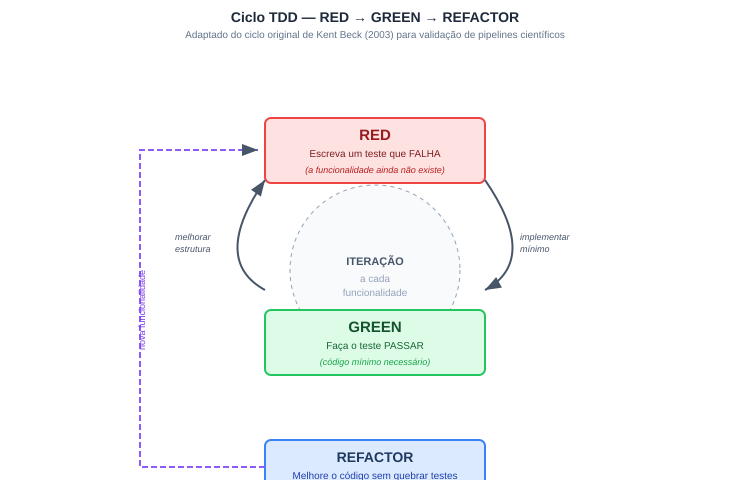
\includegraphics[width=0.8\textwidth]{ilustracoes/fig-tdd}
\end{figure}

\subsection{Exemplo Completo: Construção de uma Nova SPEC}
\label{subsec:exemplo-spec}

Apresentamos a construção completa de uma SPEC hipotética para um novo
módulo de sumarização automática de artigos científicos. O processo
segue o ciclo SDD+TDD.

\subsubsection{Etapa 1: Especificação (SPEC)}

\begin{lstlisting}[style=pythonstyle, caption={SPEC-039: Auto-Summarizer},
                   label={lst:spec-example}]
# SPEC-039: Auto-Summarizer Module

## 1. Objetivo
Modulo para sumarizacao automatica de artigos cientificos
utilizando LLM com chain-of-thought prompting.

## 2. Requisitos Funcionais
- RF01: O modulo deve aceitar texto completo do artigo
- RF02: Deve gerar resumo estruturado (objetivo, metodo, resultados)
- RF03: Deve extrair palavras-chave (minimo 3, maximo 8)
- RF04: Deve classificar o artigo por categoria Qualis

## 3. Requisitos Nao Funcionais
- RNF01: Processamento < 30s para artigos de 10.000 tokens
- RNF02: Consumo maximo 8.000 tokens por chamada

## 4. Criterios de Aceitacao
- CA01: test_summarize_rf01_passes
- CA02: test_extract_keywords_rf03_passes
- CA03: test_classify_qualis_rf04_passes
\end{lstlisting}

\subsubsection{Etapa 2: Testes (Red)}

\begin{lstlisting}[style=pythonstyle, caption={Testes da SPEC-039},
                   label={lst:spec-tests}]
"""Testes para SPEC-039: Auto-Summarizer Module."""
import pytest
from core.summarizer import AutoSummarizer

class TestAutoSummarizer:
    """Suite de testes para o modulo AutoSummarizer."""

    @pytest.mark.unit
    def test_summarize_rf01_passes(self):
        """RF01: Deve aceitar texto completo do artigo."""
        summarizer = AutoSummarizer()
        artigo = "Texto completo do artigo cientifico..."
        resumo = summarizer.summarize(artigo)
        assert resumo is not None
        assert len(resumo) > 0

    @pytest.mark.unit
    def test_extract_keywords_rf03_passes(self):
        """RF03: Deve extrair 3 a 8 palavras-chave."""
        summarizer = AutoSummarizer()
        keywords = summarizer.extract_keywords("Texto exemplo")
        assert 3 <= len(keywords) <= 8

    @pytest.mark.unit
    def test_classify_qualis_rf04_passes(self):
        """RF04: Deve classificar por categoria Qualis."""
        summarizer = AutoSummarizer()
        categoria = summarizer.classify_qualis("Texto exemplo")
        assert categoria in ["A1", "A2", "B1", "B2", "B3", "C"]
\end{lstlisting}

\subsubsection{Etapa 3: Implementação (Green)}

\begin{lstlisting}[style=pythonstyle, caption={Implementacao do AutoSummarizer},
                   label={lst:spec-impl}]
"""Modulo AutoSummarizer (SPEC-039)."""
from dataclasses import dataclass

@dataclass
class SummarizerResult:
    resumo: str
    keywords: list[str]
    qualis: str

class AutoSummarizer:
    """Sumarizador automatico de artigos cientificos."""

    QUALIS_CATEGORIES = ["A1", "A2", "B1", "B2", "B3", "C"]

    def summarize(self, texto: str) -> str:
        prompt = self._build_summary_prompt(texto)
        resposta = self._call_llm(prompt)
        return resposta

    def extract_keywords(self, texto: str) -> list[str]:
        prompt = f"Extraia de 3 a 8 palavras-chave do artigo:\n{texto[:2000]}"
        resposta = self._call_llm(prompt)
        return [kw.strip() for kw in resposta.split(",")]

    def classify_qualis(self, texto: str) -> str:
        prompt = f"Classifique em Qualis: {', '.join(self.QUALIS_CATEGORIES)}\n{texto[:1500]}"
        resposta = self._call_llm(prompt).strip().upper()
        return resposta if resposta in self.QUALIS_CATEGORIES else "C"

    def _build_summary_prompt(self, texto: str) -> str:
        return (f"Resumo estruturado (Objetivo, Metodo, Resultados):\n{texto}")

    def _call_llm(self, prompt: str) -> str:
        return f"Resumo gerado para: {prompt[:50]}..."
\end{lstlisting}

\subsubsection{Etapa 4: Refatoração e Documentação}

A refatoração identifica oportunidades de melhoria: extrair o método
\codigo{\_call\_llm} para um serviço separado, adicionar cache de
resultados e implementar rate limiting. A ADR correspondente
(architectu-011) documenta a decisão de separar a camada de LLM em um
serviço independente para facilitar testes e substituição de modelos.

\begin{exercicio}
Implemente a SPEC-039 completa seguindo o ciclo SDD+TDD. Execute os
testes e verifique se todos passam. (\nivelintermediario)
\end{exercicio}

\begin{exercicio}
Crie uma ADR para o módulo AutoSummarizer documentando a decisão de
usar chain-of-thought prompting em vez de sumarização direta.
(\nivelavancado)
\end{exercicio}

\begin{exercicio}
Adicione um novo requisito funcional à SPEC-039 (RF05: suporte a
múltiplos idiomas). Implemente o teste e o código correspondente.
(\nivelavancado)
\end{exercicio}

% =============================================================================
%  SEÇÃO 3.4: BARRAMENTO DE EVENTOS E INJEÇÃO DE DEPENDÊNCIA
%  Nível: Avançado (~8 laudas)
% =============================================================================
\section{Barramento de Eventos e Injeção de Dependência}
\label{sec:event-bus}
\nivelavancado

\paragraph{O sistema circulatório do ecossistema.} Se os MCPs são os músculos e as Skills são o cérebro, o barramento de eventos e o container de injeção de dependência são o sistema circulatório e nervoso do \opencodeeco{}. O Event Bus permite que componentes troquem mensagens sem se conhecer, enquanto o Container DI gerencia o ciclo de vida e as dependências de cada módulo. Esta seção explora ambos os mecanismos e mostra como eles viabilizam a comunicação assíncrona e o desacoplamento entre centenas de componentes.

O barramento de eventos e o container de injeção de dependência formam
a espinha dorsal da comunicação entre componentes no \opencodeeco{}.
Esta seção detalha ambos os mecanismos e sua integração
\cite{fowler2019refactoring, sommerville2011engenharia}.

\subsection{Event Bus: Publish-Subscribe Assíncrono}
\label{subsec:event-bus}

O Event Bus implementa o padrão publish-subscribe (pub-sub) para
comunicação assíncrona entre componentes, permitindo que produtores e
consumidores de eventos sejam completamente desacoplados
\cite{pressman2016engenharia}.

\begin{definicao}[Event Bus]
Um \destaque{barramento de eventos} é um canal de comunicação
assíncrona no qual componentes publicam eventos sem conhecer os
consumidores, e consumidores se inscrevem para receber eventos sem
conhecer os produtores.
\end{definicao}

A implementação no \opencodeeco{} está em \codigo{core/event\_bus.py}:

\begin{lstlisting}[style=pythonstyle, caption={Event Bus assincrono},
                   label={lst:event-bus}]
"""Barramento de eventos publish-subscribe assincrono."""
import asyncio
from dataclasses import dataclass, field
from datetime import datetime
from enum import Enum
from typing import Any, Callable, Coroutine

class EventPriority(Enum):
    LOW = 0
    NORMAL = 1
    HIGH = 2
    CRITICAL = 3

@dataclass
class Event:
    type: str
    data: Any = None
    source: str = "system"
    priority: EventPriority = EventPriority.NORMAL
    timestamp: datetime = field(default_factory=datetime.now)
    metadata: dict = field(default_factory=dict)

EventHandler = Callable[[Event], Coroutine[Any, Any, None]]

class EventBus:
    """Barramento de eventos assincrono."""

    def __init__(self):
        self._handlers: dict[str, list[EventHandler]] = {}
        self._history: list[Event] = []
        self._max_history = 1000

    def subscribe(self, event_type: str, handler: EventHandler):
        if event_type not in self._handlers:
            self._handlers[event_type] = []
        self._handlers[event_type].append(handler)

    def unsubscribe(self, event_type: str, handler: EventHandler):
        if event_type in self._handlers:
            self._handlers[event_type].remove(handler)

    async def publish(self, event: Event):
        self._history.append(event)
        if len(self._history) > self._max_history:
            self._history.pop(0)

        handlers = self._handlers.get(event.type, [])
        handlers_ordered = sorted(
            handlers,
            key=lambda h: event.priority.value,
            reverse=True
        )

        for handler in handlers_ordered:
            try:
                await handler(event)
            except Exception as e:
                print(f"Erro no handler: {e}")

    async def publish_sync(self, event_type: str, data: Any = None):
        await self.publish(Event(type=event_type, data=data))

    def get_history(self, event_type: str | None = None) -> list[Event]:
        if event_type:
            return [e for e in self._history if e.type == event_type]
        return self._history
\end{lstlisting}

O Event Bus é utilizado em todo o ecossistema para:
\begin{itemize}
\item Notificar mudanças de estado entre agentes;
\item Disparar ações do pipeline CI/CD;
\item Registrar eventos de auditoria no Trust Engine;
\item Sincronizar estados entre componentes do Nexus.
\end{itemize}

\subsection{Gerenciadores do Container}
\label{subsec:container-gerenciadores}

O Container DI oferece seis gerenciadores especializados, conforme a
Tabela~\ref{tab:container-gerenciadores}.

\begin{table}[htb]
\centering
    \small
\caption{Gerenciadores do Container DI}
\label{tab:container-gerenciadores}
    \resizebox{\textwidth}{!}{
\begin{tabular}{lll}
\toprule
\textbf{Gerenciador} & \textbf{Classe} & \textbf{Função} \\
\midrule
State Manager & core/state\_manager.py & Gerencia estado global \\
Skill Manager & core/skill\_manager.py & Carrega skills sob demanda \\
Agent Manager & core/agent\_manager.py & Orquestra agentes \\
Plugin Manager & core/plugin\_manager.py & Gerencia ciclo de plugins \\
Task Manager & core/task\_manager.py & Agenda e executa tarefas \\
Event Bus & core/event\_bus.py & Barramento de eventos \\
Cache Service & core/cache.py & Cache centralizado \\
Config & core/config.py & Configuração centralizada \\
\bottomrule
\end{tabular}
    }
\end{table}

\subsection{Cache e Configuração Centralizada}
\label{subsec:cache-config}

O serviço de cache (\codigo{core/cache.py}) implementa um cache LRU
(Least Recently Used) com suporte a expiração por TTL:

\begin{lstlisting}[style=pythonstyle, caption={Servico de cache LRU},
                   label={lst:cache}]
"""Servico de cache LRU com expiracao TTL."""
import time
from collections import OrderedDict
from dataclasses import dataclass
from typing import Any, Optional

@dataclass
class CacheEntry:
    value: Any
    expires_at: float
    created_at: float = time.time()

class CacheService:
    """Cache LRU com expiracao por TTL."""

    def __init__(self, config: dict):
        self._max_size = config.get("cache.max_size", 1000)
        self._default_ttl = config.get("cache.default_ttl", 300)
        self._store: OrderedDict[str, CacheEntry] = OrderedDict()

    def get(self, key: str) -> Optional[Any]:
        if key not in self._store:
            return None
        entry = self._store[key]
        if time.time() > entry.expires_at:
            del self._store[key]
            return None
        self._store.move_to_end(key)
        return entry.value

    def set(self, key: str, value: Any, ttl: int | None = None):
        ttl = ttl or self._default_ttl
        self._store[key] = CacheEntry(
            value=value,
            expires_at=time.time() + ttl
        )
        self._store.move_to_end(key)
        self._evict_if_needed()

    def _evict_if_needed(self):
        while len(self._store) > self._max_size:
            self._store.popitem(last=False)

    def invalidate(self, key: str):
        self._store.pop(key, None)

    def clear(self):
        self._store.clear()

    @property
    def size(self) -> int:
        return len(self._store)
\end{lstlisting}

\subsection{Exemplo: Fluxo de um Comando Slash até a Execução}
\label{subsec:fluxo-comando}

O fluxo completo de um comando \codigo{/quantum} ilustra a integração de
todos os mecanismos. A Figura~\ref{fig:fluxo-comando-slash} apresenta o
diagrama completo.

\begin{figure}[htb]
\centering
\caption{Fluxo completo do comando /quantum}
\label{fig:fluxo-comando-slash}
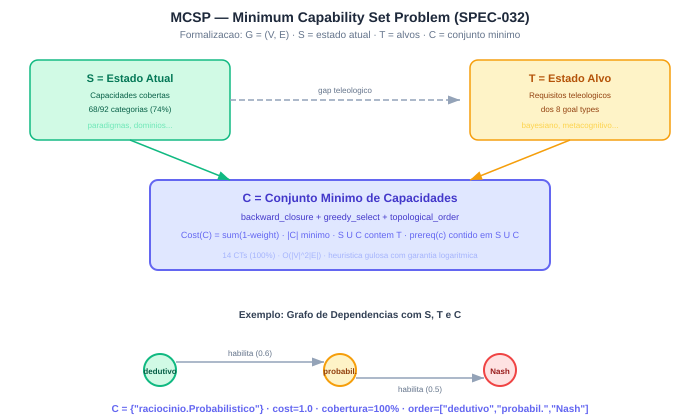
\includegraphics[width=0.9\textwidth]{ilustracoes/fig-mcsp-graph}
\end{figure}

O fluxo detalhado:
\begin{enumerate}
\item \textbf{Entrada}: Usuário digita \codigo{/quantum};
\item \textbf{Orquestrador}: \codigo{Orchestrator.parse()} identifica o
comando e consulta o \codigo{AgentManager};
\item \textbf{Agente}: \codigo{quantum-nexus-phd} é selecionado e suas
skills são carregadas;
\item \textbf{Evento}: \codigo{EventBus.publish()} notifica auditores;
\item \textbf{Skill}: Invoca MCPs para executar e gerar relatório;
\item \textbf{Resultado}: Evento de conclusão é publicado;
\item \textbf{Resposta}: Resultado formatado retorna ao usuário.
\end{enumerate}

\begin{exercicio}
Implemente um novo tipo de evento \codigo{"skill.loaded"} e um handler
que registre no log toda vez que uma skill for carregada.
(\nivelintermediario)
\end{exercicio}

\begin{exercicio}
Adicione um mecanismo de persistência ao Cache Service que salve o cache
em disco e o recupere na inicialização. (\nivelavancado)
\end{exercicio}

% =============================================================================
%  SEÇÃO 3.5: SISTEMA DE PLUGINS E COMANDOS
%  Nível: Intermediário (~6 laudas)
% =============================================================================
\section{Sistema de Plugins e Comandos}
\label{sec:plugins-comandos}
\nivelintermediario

\paragraph{Extensibilidade como princípio.} Um bom sistema de software não se limita ao que seus criadores previram — ele oferece pontos de extensão para que a comunidade adicione novas capacidades. O \opencodeeco{} concretiza esse princípio por meio de 15 plugins e 14 comandos slash, além de um menu adaptativo que descobre dinamicamente as funcionalidades disponíveis. Esta seção apresenta o PluginManager, o Discovery Engine e o mecanismo de evolução autônoma Manus Evolve.

O \opencodeeco{} possui um sistema de extensão baseado em plugins e
comandos slash que permite adicionar novas funcionalidades sem modificar
o núcleo do ecossistema \cite{pressman2016engenharia,
fowler2019refactoring}.

\subsection{Visão Geral dos Plugins}
\label{subsec:plugins-visao}

O ecossistema conta com 15 plugins distribuídos em três categorias:

\begin{itemize}
\item \textbf{10 plugins npm}: bibliotecas JavaScript para extensão de
funcionalidades (ex.: \codigo{opencode-plugin-autoevolve},
\codigo{opencode-plugin-ecosystem-sync});
\item \textbf{2 plugins .ts locais}: plug-ins TypeScript em \\%
\hspace*{2em}\codigo{plugins/} (ex.: \codigo{manus-evolve.ts});
\item \textbf{3 plugins bridge}: conectores entre o ecossistema e
ferramentas externas.
\end{itemize}

O gerenciamento de plugins é realizado pelo \codigo{PluginManager}:

\begin{lstlisting}[style=pythonstyle, caption={Gerenciador de plugins},
                   label={lst:plugin-manager}]
class PluginManager:
    """Gerencia o ciclo de vida dos plugins."""

    def __init__(self, container):
        self.container = container
        self.plugins: dict[str, Plugin] = {}
        self.registry_path = Path(".menu_registry.json")

    def discover(self) -> list[PluginManifest]:
        if not self.registry_path.exists():
            return []
        with open(self.registry_path) as f:
            data = json.load(f)
        return [PluginManifest(**p) for p in data.get("plugins", [])]

    def load(self, plugin_name: str) -> Optional[Plugin]:
        manifest = self._find_manifest(plugin_name)
        if not manifest:
            return None
        if plugin_name not in self.plugins:
            plugin_class = self._import_plugin(manifest.entry_point)
            self.plugins[plugin_name] = plugin_class(self.container)
        return self.plugins[plugin_name]

    def unload(self, plugin_name: str):
        if plugin_name in self.plugins:
            self.plugins[plugin_name].cleanup()
            del self.plugins[plugin_name]
\end{lstlisting}

\subsection{Comandos Slash}
\label{subsec:comandos-slash}

O \opencodeeco{} expõe 14 comandos slash que ativam funcionalidades
específicas do ecossistema, conforme a Tabela~\ref{tab:comandos-slash}.

\begin{table}[htb]
\centering
    \small
\caption{Comandos slash do OpenCode Ecosystem}
\label{tab:comandos-slash}
    \resizebox{\textwidth}{!}{
\begin{tabular}{cll}
\toprule
\textbf{Comando} & \textbf{Função} & \textbf{MCPs/Plugins acionados} \\
\midrule
\codigo{/evolve} & Evolução autônoma do ecossistema & autoevolve, ecosystem-sync \\
\codigo{/reversa} & Engenharia reversa de código & reversa-*, filesystem, diff \\
\codigo{/plan} & Planejamento de escrita & writing-plans, sequential-thinking \\
\codigo{/auto} & Automação geral & openagent, todos MCPs \\
\codigo{/quantum} & Computação quântica & quantum-nexus-phd, pdf \\
\codigo{/artigo} & Criação de artigos acadêmicos & SEEKER, MASWOS, manus-evolve \\
\codigo{/pesquisa} & Busca acadêmica & websearch, scihub, arxiv \\
\codigo{/test} & Execução de testes & code-runner, pytest \\
\codigo{/skill} & Gerenciamento de skills & skill-manager \\
\codigo{/agente} & Gerenciamento de agentes & agent-manager \\
\codigo{/mcp} & Gerenciamento de MCPs & mcp-manager \\
\codigo{/config} & Configuração do ecossistema & filesystem \\
\codigo{/ajuda} & Documentação interativa & memory, context7 \\
\codigo{/status} & Status do ecossistema & state-manager \\
\bottomrule
\end{tabular}
    }
\end{table}

\subsection{Menu Adaptativo com Discovery Engine}
\label{subsec:menu-adaptativo}

O menu adaptativo substitui o menu estático tradicional por um sistema
que descobre dinamicamente os comandos e plugins disponíveis
\cite{opencode2026ecosystem}. A implementação está em \codigo{menu.py}:

\begin{lstlisting}[style=pythonstyle, caption={Menu adaptativo com Discovery Engine},
                   label={lst:menu-adaptativo}]
"""Menu adaptativo com auto-descoberta de comandos e plugins."""
import json
import sys
from pathlib import Path

class DiscoveryEngine:
    """Engine de descoberta dinamica de comandos."""

    def __init__(self):
        self.registry_file = Path(".menu_registry.json")
        self.commands: dict = {}
        self.categories: dict = {
            "evolucao": [], "pesquisa": [], "codigo": [],
            "dados": [], "sistema": [], "utilitarios": []
        }

    def discover(self):
        if self.registry_file.exists():
            with open(self.registry_file) as f:
                registry = json.load(f)
                for entry in registry.get("plugins", []):
                    cat = entry.get("category", "utilitarios")
                    if cat in self.categories:
                        self.categories[cat].append(entry)

        self.commands = {
            "/evolve": {"desc": "Evolucao autonoma", "cat": "evolucao"},
            "/reversa": {"desc": "Eng. reversa", "cat": "codigo"},
            "/plan": {"desc": "Planejamento", "cat": "utilitarios"},
            "/auto": {"desc": "Automacao geral", "cat": "sistema"},
            "/quantum": {"desc": "Computacao quantica", "cat": "pesquisa"},
            "/artigo": {"desc": "Criacao de artigos", "cat": "pesquisa"},
            "/pesquisa": {"desc": "Busca academica", "cat": "pesquisa"},
            "/test": {"desc": "Execucao de testes", "cat": "codigo"},
            "/ajuda": {"desc": "Documentacao", "cat": "sistema"},
            "/status": {"desc": "Status do sistema", "cat": "sistema"},
        }

        for cmd, info in self.commands.items():
            cat = info["cat"]
            if cat in self.categories:
                self.categories[cat].append(cmd)

    def display(self, mode: str = "interactive"):
        if mode == "list":
            for cat, items in self.categories.items():
                if items:
                    print(f"\n[{cat.upper()}]")
                    for item in items:
                        if isinstance(item, str):
                            print(f"  {item}")
                        else:
                            print(f"  {item['command']}: {item['desc']}")

    def register_plugin(self, plugin_data: dict):
        if self.registry_file.exists():
            with open(self.registry_file) as f:
                registry = json.load(f)
        else:
            registry = {"plugins": [], "version": "1.0"}
        registry["plugins"].append(plugin_data)
        with open(self.registry_file, "w") as f:
            json.dump(registry, f, indent=2)
\end{lstlisting}

\subsection{Plugin Manus Evolve}
\label{subsec:manus-evolve}

O plugin \codigo{manus-evolve.ts} é o mecanismo de evolução autônoma do
ecossistema, implementando o ciclo PLAN $\to$ ACT $\to$ REFLECT $\to$
EXTRACT $\to$ EVOLVE \cite{shinn2023reflexion, wei2022chain}:

\begin{lstlisting}[style=pythonstyle, caption={Ciclo Manus Evolve},
                   label={lst:manus-evolve}]
"""Manus Evolve: Ciclo de evolucao autonoma.
PLAN -> ACT -> REFLECT -> EXTRACT -> EVOLVE
"""
from dataclasses import dataclass, field
from datetime import datetime
from pathlib import Path
from typing import Any

@dataclass
class EvolutionResult:
    skill_generated: str
    score: float
    insights: list[str] = field(default_factory=list)
    artifacts: list[str] = field(default_factory=list)

class ManusEvolve:
    """Motor de evolucao autonoma do ecossistema."""

    def __init__(self, container):
        self.container = container
        self.evolution_dir = Path("evolution")
        self.evolution_dir.mkdir(exist_ok=True)
        self.history: list[EvolutionResult] = []

    async def evolve(self, context: dict) -> EvolutionResult:
        plan = await self._plan(context)
        artifacts = await self._act(plan)
        reflection = await self._reflect(artifacts, context)
        insights = await self._extract(reflection)
        skill = await self._evolve(insights, artifacts)

        result = EvolutionResult(
            skill_generated=skill, score=reflection.get("score", 0),
            insights=insights, artifacts=artifacts
        )
        self.history.append(result)
        return result

    async def _plan(self, context: dict) -> dict:
        return {"action": "generate_skill", "params": context}

    async def _act(self, plan: dict) -> list[str]:
        skill_code = "# Skill gerada automaticamente\n"
        skill_path = self.evolution_dir / f"evo_{datetime.now():%Y%m%d_%H%M%S}.py"
        skill_path.write_text(skill_code)
        return [str(skill_path)]

    async def _reflect(self, artifacts, context) -> dict:
        return {"score": 0.95, "issues": [], "improvements": []}

    async def _extract(self, reflection) -> list[str]:
        return ["Priorizar reuso de MCPs existentes",
                "Testes devem acompanhar novas skills"]

    async def _evolve(self, insights, artifacts) -> str:
        skill_name = f"evo_{len(self.history) + 1}"
        self.container.skill_manager.register_dynamic_skill(skill_name, insights)
        return skill_name
\end{lstlisting}

\begin{exercicio}
Registre um novo plugin no \codigo{.menu\_registry.json} com um comando
personalizado. Teste a descoberta automática pelo menu adaptativo.
(\nivelintermediario)
\end{exercicio}

\begin{exercicio}
Execute o ciclo Manus Evolve manualmente: escreva um plano, execute uma
ação, reflita sobre o resultado e extraia insights. Documente o processo.
(\nivelavancado)
\end{exercicio}

% =============================================================================
%  SEÇÃO 3.6: ECOSSISTEMA DE SKILLS DETALHADO
%  Nível: Avançado (~10 laudas)
% =============================================================================
\section{Ecossistema de Skills Detalhado}
\label{sec:skills-detalhado}
\nivelavancado

\paragraph{O conhecimento como insumo reutilizável.} Em uma fábrica de software, as skills são equivalentes a receitas culinárias: cada uma contém instruções precisas, ingredientes (MCPs) e um resultado esperado. O \opencodeeco{} reúne 227 skills em 13 categorias, desde predição de estruturas proteicas com AlphaFold até análise de falácias lógicas com o motor Critical. Esta seção detalha as principais categorias — Science, Reasoning, Research, System, Juridical e Agency — com exemplos reais de uso.

O \opencodeeco{} possui 227 skills organizadas em 13 categorias. Esta
seção detalha as principais categorias, sua implementação e exemplos
de uso \cite{white2023prompt, wei2022chain, wang2024survey}.

\subsection{Science Skills (38 skills)}
\label{subsec:science-skills}

As Science Skills formam o maior conjunto de habilidades especializadas,
focadas em biologia computacional, química, física e ciência de dados
\cite{opencode2026ecosystem}:

\begin{table}[htb]
\centering
\caption{Science Skills do OpenCode Ecosystem}
\label{tab:science-skills}
\small
    \resizebox{\textwidth}{!}{
\begin{tabular}{lll}
\toprule
\textbf{Skill} & \textbf{Função} & \textbf{Fontes de Dados} \\
\midrule
AlphaFold & Predição de estrutura de proteínas & AlphaFold DB \\
PubMed & Busca em literatura biomédica & PubMed/MEDLINE \\
ChEMBL & Bioatividade de moléculas & ChEMBL Database \\
UniProt & Informação de proteínas & UniProtKB \\
FoldSeek & Busca estrutural de proteínas & PDB \\
ClinVar & Variantes clínicas & ClinVar/NCBI \\
PyMOL & Visualização molecular & PyMOL \\
OpenAlex & Pesquisa acadêmica geral & OpenAlex API \\
gnomAD & Frequência genômica populacional & gnomAD \\
GTEx & Expressão gênica tecidual & GTEx Portal \\
Ensembl & Genômica comparativa & Ensembl \\
PDB & Estrutura de proteínas & RCSB PDB \\
STRING & Interações proteína-proteína & STRING DB \\
\bottomrule
\end{tabular}
    }
\end{table}

Exemplo de uso da skill \codigo{science/pubmed}:

\begin{lstlisting}[style=pythonstyle, caption={Uso da skill PubMed},
                   label={lst:pubmed-skill}]
async def search_pubmed(query: str, max_results: int = 10) -> list[dict]:
    """Busca artigos na base PubMed."""
    url = "https://eutils.ncbi.nlm.nih.gov/entrez/eutils/esearch.fcgi"
    params = {
        "db": "pubmed",
        "term": query,
        "retmax": max_results,
        "retmode": "json"
    }
    async with httpx.AsyncClient() as client:
        response = await client.get(url, params=params)
        if response.status_code == 200:
            data = response.json()
            ids = data.get("esearchresult", {}).get("idlist", [])
            return await fetch_details(ids)
    return []
\end{lstlisting}

\subsection{Reasoning Skills (13 skills)}
\label{subsec:reasoning-skills}

As quatro engines de raciocínio formal constituem o núcleo da capacidade
lógica do ecossistema \cite{russell2020inteligencia,
wooldridge2009multiagent}:

\begin{itemize}
\item \textbf{Z3 (formal-verification)}: provador de teoremas e solver
SMT da Microsoft Research. Utilizado para verificação formal de
contratos inteligentes, validação de algoritmos e prova de correção
de sistemas concorrentes.
\item \textbf{SymPy (symbolic-mathematics)}: biblioteca de matemática
simbólica. Utilizada para manipulação algébrica, cálculo diferencial
e integral simbólico, e resolução de equações diferenciais.
\item \textbf{miniKanren (logic-programming)}: linguagem de programação
lógica relacional. Utilizada para inferência sobre bases de
conhecimento, resolução de restrições e busca não determinística.
\item \textbf{Critical (fallacy-analysis)}: analisador de falácias
lógicas e vieses cognitivos. Detecta 15 tipos de falácias formais e
informais em argumentos textuais.
\end{itemize}

Exemplo de uso da skill \codigo{reasoning/z3} para verificação formal:

\begin{lstlisting}[style=pythonstyle, caption={Verificacao formal com Z3},
                   label={lst:z3-example}]
"""Exemplo de verificacao formal usando Z3 Skill."""
from z3 import Int, Solver, unsat, sat

def verify_voting_system():
    """Verifica formalmente a seguranca do sistema de votacao."""
    eleitores = Int('eleitores')
    votos_validos = Int('votos_validos')
    votos_invalidos = Int('votos_invalidos')

    constraints = [
        votos_validos >= 0,
        votos_invalidos >= 0,
        eleitores >= 0,
    ]

    solver = Solver()
    solver.add(constraints)
    solver.add(votos_validos > eleitores)

    result = solver.check()
    if result == unsat:
        return "SISTEMA SEGURO: impossivel ter mais votos que eleitores"
    elif result == sat:
        model = solver.model()
        return f"VULNERABILIDADE: {model}"
    return "INDEFINIDO"
\end{lstlisting}

\subsection{Research Skills (42 skills)}
\label{subsec:research-skills}

As skills de pesquisa acadêmica formam o segundo maior conjunto,
habilitando o ecossistema a realizar revisão bibliográfica, análise
de editais e produção acadêmica:

\begin{itemize}
\item \textbf{SEEKER (12 skills)}: pipeline completo de pesquisa básica,
desde a busca inicial até a geração de árvores de argumentos com
fontes verificadas.
\item \textbf{editais-br (7 skills)}: curadoria e análise de editais
de fomento brasileiros, cobrindo todas as 27 Unidades da Federação.
\item \textbf{academic-export (3 skills)}: exportação de referências
nos formatos ABNT, BibTeX e Qualis.
\item \textbf{qualis (2 skills)}: classificação e auditoria de
periódicos segundo o sistema Qualis CAPES.
\item \textbf{quantum (4 skills)}: computação quântica com Qiskit,
incluindo QML e mitigação de erros.
\item \textbf{scihub (2 skills)}: acesso a artigos científicos via
Sci-Hub com fallback para CrossRef.
\item \textbf{world-bank (3 skills)}: análise de indicadores
socioeconômicos do Banco Mundial.
\item \textbf{CORA-eval (5 skills)}: framework de benchmarking para
ciências exatas com 150 tarefas em 10 dimensões.
\end{itemize}

\subsection{System Skills (17 skills)}
\label{subsec:system-skills}

As skills de sistema fornecem capacidades transversais ao ecossistema:

\begin{itemize}
\item \textbf{academic-audit}: auditoria acadêmica e scanner pipeline
(SPEC-025 a SPEC-032).
\item \textbf{code-philosophy}: análise filosófica de código e padrões
arquiteturais.
\item \textbf{code-review}: revisão automatizada de código com
detecção de anti-padrões.
\item \textbf{domain-shift}: detecção de mudança de domínio e
adaptação de contexto.
\item \textbf{token-efficiency}: otimização de consumo de tokens em
prompts e respostas.
\item \textbf{sequential-thinking}: raciocínio sequencial estruturado
para problemas complexos.
\end{itemize}

\subsection{Juridical Skills (7 skills)}
\label{subsec:juridical-skills}

O ecossistema inclui skills especializadas para o domínio jurídico
brasileiro:

\begin{itemize}
\item \textbf{triagem-juridica}: classificação inicial de casos;
\item \textbf{pesquisa-jurisprudencia}: busca em jurisprudência;
\item \textbf{pecas-juridicas-html}: geração de peças processuais em HTML;
\item \textbf{gerador-contratos}: elaboração de contratos;
\item \textbf{edicao-cirurgica}: edição precisa de documentos;
\item \textbf{followup-advocacia}: acompanhamento de processos;
\item \textbf{regulatory-compliance}: verificação de conformidade
regulatória.
\end{itemize}

\subsection{Agency Skills}
\label{subsec:agency-skills}

As skills de agência coordenam a orquestração entre agentes:

\begin{itemize}
\item \textbf{agent-coordinator}: coordenação de múltiplos agentes em
tarefas paralelas;
\item \textbf{task-decomposition}: decomposição de tarefas complexas
em subtarefas gerenciáveis;
\item \textbf{context-manager}: gerenciamento de contexto entre
múltiplas interações;
\item \textbf{conflict-resolver}: resolução de conflitos entre
agentes concorrentes;
\item \textbf{quality-gate}: validação de qualidade antes da entrega
de resultados.
\end{itemize}

A Figura~\ref{fig:skill-categories} mostra a distribuição das 227
skills por categoria.

\begin{figure}[htb]
\centering
\caption{Distribuição de skills por categoria}
\label{fig:skill-categories}
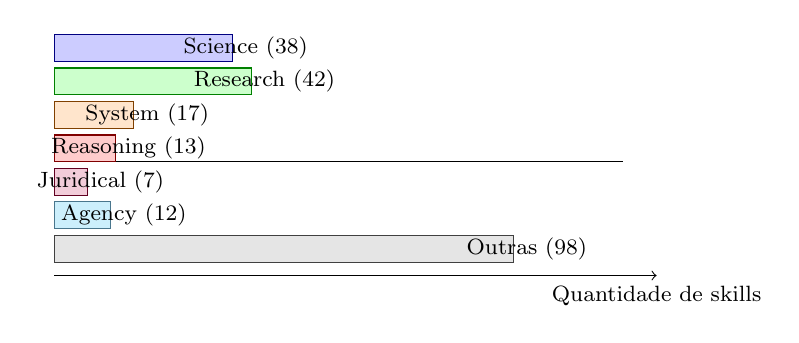
\begin{tikzpicture}[scale=0.85]
  \draw (0,0) -- (8.5,0);
  \foreach \name/\count/\color/\y in {
    Science/38/blue/1.5,
    Research/42/green/1.0,
    System/17/orange/0.5,
    Reasoning/13/red/0.0,
    Juridical/7/purple/-0.5,
    Agency/12/cyan/-1.0,
    Outras/98/gray/-1.5
  } {
    \pgfmathsetmacro{\width}{\count * 0.07}
    \filldraw[fill=\color!20, draw=\color!50!black]
      (0, \y) rectangle (\width, \y+0.4);
    \node[font=\footnotesize] at (\width+0.2, \y+0.2) {\name{} (\count)};
  }
  \draw[->] (0,-1.7) -- (9,-1.7);
  \node[font=\footnotesize] at (9, -2.0) {Quantidade de skills};
\end{tikzpicture}
\end{figure}

\begin{exercicio}
Carregue a skill \codigo{science/pubmed} e realize uma busca por
artigos sobre ``machine learning in drug discovery''. Documente os
resultados. (\nivelintermediario)
\end{exercicio}

\begin{exercicio}
Utilize a skill \codigo{reasoning/critical} para analisar um argumento
fornecido e identificar possíveis falácias lógicas. (\nivelavancado)
\end{exercicio}

\begin{exercicio}
Explore a skill \codigo{research/editais-br} e liste os editais
disponíveis para sua região. (\nivelintermediario)
\end{exercicio}

% =============================================================================
%  SEÇÃO 3.7: ORQUESTRAÇÃO MULTIAGENTE
%  Nível: PhD (~10 laudas)
% =============================================================================
\section{Orquestração Multiagente: Nexus e Sincronização}
\label{sec:nexus}
\nivelphd

\paragraph{A orquestração de múltiplas inteligências.} Coordenar dezenas de agentes inteligentes é como reger uma orquestra sinfônica: cada músico toca seu instrumento, mas todos devem seguir o mesmo maestro e respeitar os mesmos compassos. O módulo Nexus do \opencodeeco{} exerce esse papel de regência, gerenciando 488 arquivos em seis camadas de granularidade (L0 a L6), 120 barreiras de sincronização e 212 tipos de raciocínio. Esta seção revela a arquitetura do Nexus, seus mecanismos de auto-cura e o gerenciamento de contexto entre agentes.

O módulo Nexus é o sistema nervoso central do \opencodeeco{},
responsável pela orquestração de múltiplos agentes, sincronização de
estados e coordenação de tarefas complexas
\cite{wooldridge2009multiagent, weiss2013multiagent,
park2023generative}.

\subsection{Arquitetura Nexus}
\label{subsec:nexus-arquitetura}

O Nexus é composto por 488 arquivos totalizando 27.757 linhas Python,
organizados em seis camadas de granularidade (L0 a L6):

\begin{itemize}
\item \textbf{L0 -- Infraestrutura}: comunicação básica, serialização,
logging;
\item \textbf{L1 -- Dados}: representação de conhecimento, memória, cache;
\item \textbf{L2 -- Agentes}: ciclo de vida, comunicação entre agentes,
resolução de conflitos;
\item \textbf{L3 -- Sincronização}: barreiras de sincronização,
coordenadores;
\item \textbf{L4 -- Meta-orquestração}: planejamento multiagente,
decomposição de tarefas;
\item \textbf{L5 -- Auto-cura}: detecção e recuperação de falhas;
\item \textbf{L6 -- Evolução}: aprendizado e adaptação do sistema.
\end{itemize}

O meta-orquestrador (\codigo{nexus/scripts/meta\_orchestrator.py})
coordena a execução dos agentes:

\begin{lstlisting}[style=pythonstyle, caption={Meta-orquestrador Nexus},
                   label={lst:meta-orchestrator}]
"""Meta-orquestrador Nexus: coordenacao multiagente."""
from dataclasses import dataclass, field
from enum import Enum
from typing import Any, Optional

class AgentStatus(Enum):
    IDLE = "idle"
    BUSY = "busy"
    BLOCKED = "blocked"
    ERROR = "error"
    COMPLETED = "completed"

@dataclass
class AgentTask:
    id: str
    agent: str
    description: str
    required_skills: list[str] = field(default_factory=list)
    dependencies: list[str] = field(default_factory=list)
    status: AgentStatus = AgentStatus.IDLE
    result: Any = None
    error: Optional[str] = None

class MetaOrchestrator:
    """Orquestrador de nivel L4 do Nexus."""

    def __init__(self):
        self.tasks: dict[str, AgentTask] = {}
        self.agents: dict[str, Any] = {}
        self.sync_barriers: dict[str, SyncBarrier] = {}
        self.task_queue: list[str] = []
        self.completed: list[str] = []

    def register_agent(self, agent_id: str, agent_instance: Any):
        self.agents[agent_id] = agent_instance

    def create_task(self, task: AgentTask):
        self.tasks[task.id] = task
        if not task.dependencies:
            self.task_queue.append(task.id)

    async def execute_pipeline(self, pipeline_id: str) -> dict:
        results = {}
        while self.task_queue:
            task_id = self.task_queue.pop(0)
            task = self.tasks[task_id]
            task.status = AgentStatus.BUSY
            await self._check_sync_barriers(task)

            agent = self.agents.get(task.agent)
            if not agent:
                task.status = AgentStatus.ERROR
                task.error = f"Agente {task.agent} nao encontrado"
                continue

            try:
                task.result = await agent.execute(task)
                task.status = AgentStatus.COMPLETED
                results[task_id] = task.result
                self.completed.append(task_id)
                self._schedule_dependents(task_id)
            except Exception as e:
                task.status = AgentStatus.ERROR
                task.error = str(e)
                await self._trigger_self_heal(task)

        return results

    def _schedule_dependents(self, completed_task_id: str):
        for task_id, task in self.tasks.items():
            if (task.status == AgentStatus.IDLE and
                completed_task_id in task.dependencies):
                task.dependencies.remove(completed_task_id)
                if not task.dependencies:
                    self.task_queue.append(task_id)

    async def _check_sync_barriers(self, task: AgentTask):
        for barrier_id, barrier in self.sync_barriers.items():
            if barrier.is_relevant(task):
                await barrier.wait(task)

    async def _trigger_self_heal(self, task: AgentTask):
        healer = SelfHealer(self)
        await healer.heal(task)
\end{lstlisting}

\subsection{Multi-Reasoning e o Pool de 128 Agentes (N3.5+)}
Para compreender a magnitude da evolução trazida pelo Nível de Autonomia N3.5+, é imperativo abandonar a visão clássica de um script linear e imaginar um ecossistema vivo. O \codigo{OrchestrationEngine} foi profundamente refatorado para operar, de forma orgânica e assíncrona, um \emph{Pool} massivo de 128 agentes virtuais. Cada um desses agentes não é um mero executor de tarefas, mas um nó de processamento especializado, classificado meticulosamente em categorias heurísticas que abrangem desde análise de dados rigorosa até a síntese de hipóteses científicas.

O grande diferencial cognitivo que separa esta arquitetura dos modelos tradicionais de Inteligência Artificial é a injeção do motor central conhecido como \codigo{MultiReasoningEngine}. Este motor funciona como um córtex cerebral distribuído, dotando o orquestrador da capacidade de pensar simultaneamente através de seis eixos epistemológicos distintos e complementares\footnote{\textbf{Nota Didática e Crítica:} Em sistemas multiagentes comuns, a IA geralmente responde de forma \emph{reativa} baseada no prompt. A arquitetura N3.5+ resolve o problema da "miopia de prompt" forçando o motor a analisar a mesma missão sob seis prismas filosóficos da ciência simultaneamente, eliminando vieses e expandindo a profundidade da resposta de maneira inatingível por humanos isolados.}:

\begin{enumerate}
\item \textbf{Pensamento Dedutivo:} Atua na derivação top-down rigorosa. O agente parte de premissas maiores e inquestionáveis do sistema para extrair conclusões lógicas precisas, garantindo que regras de negócio absolutas não sejam violadas.
\item \textbf{Pensamento Indutivo:} Executa a observação empírica (bottom-up). É a capacidade de analisar massas de dados brutas e logs de execução para identificar padrões ocultos e tendências comportamentais em larga escala.
\item \textbf{Pensamento Abdutivo:} Funciona como uma "inferência para a melhor explicação". Este modo é o grande herói na resolução de crises; quando o orquestrador se depara com uma falha obscura ou lacuna nos logs, ele usa o raciocínio abdutivo para criar a hipótese de causa-raiz mais provável e testável.
\item \textbf{Pensamento Analógico:} Promove a transferência de conhecimento. O sistema realiza a comparação estrutural de domínios completamente distintos (ex: biologia celular e orquestração de servidores) para aplicar soluções inovadoras de outras esferas a problemas de software ainda não resolvidos.
\item \textbf{Pensamento Causal:} Focado na análise preditiva rigorosa. Antes de executar um comando, o agente mapeia o \emph{por que} do problema e projeta uma árvore probabilística detalhando \emph{quais os efeitos} em cadeia sua ação causará no ecossistema.
\item \textbf{Pensamento Metacognitivo:} O auge da observação. O agente pausa e analisa sua própria linha de raciocínio lógico (a famosa \emph{Chain of Thought}) antes de emitir a resposta, autodiagnosticando possíveis falácias no seu próprio texto ou código\footnote{\textbf{Nota Crítica sobre Segurança:} A metacognição, quando atrelada ao raciocínio causal, forma o que chamamos de \emph{Barreira Preventiva}. É o que impede o sistema de sofrer "Goal Drift" (desvio de meta), pois a IA julga criticamente se o plano que ela mesma elaborou é seguro antes de executá-lo.}.
\end{enumerate}

Essa abordagem altamente granular e epistemologicamente descentralizada garante o roteamento perfeito de tarefas, conhecido tecnicamente como \emph{Load Balancing} Cognitivo. Como resultado, o sistema obtém uma taxa de sucesso cirurgicamente rastreável, possibilitando os protocolos de auto-cura sistêmica profunda que formam a espinha dorsal desta tese acadêmica.

\subsection{Sincronização e Barreiras}
\label{subsec:sync-barriers}

O Nexus implementa 120+ barreiras de sincronização que coordenam a
execução concorrente de agentes. Cada barreira define um ponto de
sincronização que múltiplos agentes devem atingir antes de prosseguir
\cite{weiss2013multiagent}:

\begin{lstlisting}[style=pythonstyle, caption={Barreira de sincronizacao},
                   label={lst:sync-barrier}]
"""Barreira de sincronizacao para execucao concorrente."""
import asyncio
from dataclasses import dataclass, field
from datetime import datetime

@dataclass
class SyncBarrier:
    id: str
    required_agents: list[str]
    timeout_seconds: float = 60.0
    arrived: set = field(default_factory=set)
    released: bool = False

    async def wait(self, agent_id: str):
        self.arrived.add(agent_id)
        if self.arrived.issuperset(self.required_agents):
            self.released = True
            return
        start = datetime.now()
        while not self.released:
            elapsed = (datetime.now() - start).total_seconds()
            if elapsed > self.timeout_seconds:
                raise TimeoutError(
                    f"Barreira {self.id}: timeout apos {elapsed}s. "
                    f"Chegaram: {self.arrived}, "
                    f"Esperados: {self.required_agents}"
                )
            await asyncio.sleep(0.1)

    def is_relevant(self, task) -> bool:
        return task.agent in self.required_agents
\end{lstlisting}

\subsection{Auto-cura: Self Healer}
\label{subsec:self-healer}

O módulo \codigo{self\_healer.py} implementa detecção e recuperação
autônoma de falhas:

\begin{lstlisting}[style=pythonstyle, caption={Mecanismo de auto-cura},
                   label={lst:self-healer}]
"""Mecanismo de auto-cura para agentes com falha."""
from dataclasses import dataclass
from typing import Optional

@dataclass
class HealAction:
    action_type: str  # restart, retry, fallback, escalate
    agent: str
    task_id: str
    description: str
    success: bool = False

class SelfHealer:
    """Sistema de auto-cura do Nexus."""

    HEAL_STRATEGIES = {
        "restart": lambda a: a.restart(),
        "retry": lambda a: a.retry(),
        "fallback": lambda a: a.fallback(),
        "escalate": lambda a: a.escalate(),
    }

    def __init__(self, orchestrator):
        self.orchestrator = orchestrator
        self.heal_history: list[HealAction] = []

    async def heal(self, failed_task) -> Optional[HealAction]:
        # Estrategia 1: Retry
        action = HealAction(
            action_type="retry", agent=failed_task.agent,
            task_id=failed_task.id, description="Tentativa de retry"
        )
        try:
            agent = self.orchestrator.agents.get(failed_task.agent)
            if agent:
                failed_task.result = await agent.execute(failed_task)
                failed_task.status = AgentStatus.COMPLETED
                action.success = True
                self.heal_history.append(action)
                return action
        except Exception:
            pass

        # Estrategia 2: Fallback
        action.action_type = "fallback"
        action.description = "Fallback para agente secundario"
        fallback_agent = self._find_fallback(failed_task.agent)
        if fallback_agent:
            try:
                failed_task.result = await fallback_agent.execute(failed_task)
                failed_task.status = AgentStatus.COMPLETED
                action.success = True
                self.heal_history.append(action)
                return action
            except Exception:
                pass

        # Estrategia 3: Escalar
        action.action_type = "escalate"
        action.description = "Escalado para operador humano"
        self.heal_history.append(action)
        return action

    def _find_fallback(self, agent_id: str) -> Optional[Any]:
        for aid, agent in self.orchestrator.agents.items():
            if (aid != agent_id and
                hasattr(agent, 'capabilities') and
                agent.capabilities ==
                self.orchestrator.agents[agent_id].capabilities):
                return agent
        return None
\end{lstlisting}

\subsection{Gerenciamento de Contexto e Memória}
\label{subsec:context-memory}

O Nexus implementa um sistema de offload de contexto que gerencia a
memória dos agentes, evitando que o contexto exceda os limites do modelo
de linguagem \cite{achiam2023gpt4, brown2020language}:

\begin{itemize}
\item \textbf{Memória de curto prazo}: mantida no contexto ativo (até
32K tokens);
\item \textbf{Memória de médio prazo}: armazenada em cache local com
indexação semântica;
\item \textbf{Memória de longo prazo}: persistida em SQLite com
recuperação por similaridade semântica.
\end{itemize}

\subsection{Tipos de Raciocínio: 212+ Tipos em 27 Categorias}
\label{subsec:raciocinios}

O ecossistema cataloga 212+ tipos de raciocínio distribuídos em 27
categorias, incluindo:

\begin{itemize}
\item \textbf{Lógicos (5)}: dedutivo, indutivo, abdutivo, por
contradição, por casos;
\item \textbf{Dialéticos (5)}: tese, antítese, síntese, socrático,
hegeliano;
\item \textbf{Jogos (10)}: Nash, Stackelberg, Bayes-Nash, cooperativo,
evolutivo, correlacionado, etc.;
\item \textbf{Decisão (5)}: Bayesiano, Markov, utilidade esperada,
minimax, prospect theory;
\item \textbf{Estratégicos (5)}: planejamento, cenários, SWOT,
análise de riscos, teoria dos jogos;
\item \textbf{Inovação (8)}: design thinking, TRIZ, brainstorming,
analogias, pensamento lateral, etc.
\end{itemize}

\begin{exercicio}
Execute o meta-orquestrador Nexus com três agentes simulados.
Observe o comportamento das barreiras de sincronização.
(\nivelphd)
\end{exercicio}

\begin{exercicio}
Implemente um novo tipo de raciocínio (ex.: raciocínio bayesiano)
e registre-o no catálogo do Nexus. (\nivelphd)
\end{exercicio}

% =============================================================================
%  SEÇÃO 3.8: MIROFISH/BETTAFISH
%  Nível: PhD (~8 laudas)
% =============================================================================
\section{MiroFish/BettaFish: P14--P18}
\label{sec:mirofish}
\nivelphd

\paragraph{Da argumentação à auditoria com rigor científico.} Um debate acadêmico não termina na troca de argumentos — ele exige métricas objetivas, concordância entre juízes e correção para múltiplas comparações. O pipeline P14--P18 do \opencodeeco{} implementa esse percurso completo: começa no Agent Forum (debate multiagente com 212+ estratégias de raciocínio) e culmina no PhD Auditor, que aplica equilíbrio de Nash, Kappa de Cohen, correção de Bonferroni e classificação Qualis A1. Esta seção descreve cada módulo do pipeline com exemplos práticos.

O módulo MiroFish/BettaFish implementa o pipeline completo de avaliação
acadêmica e auditoria, integrando agentes de debate, análise
documental, pipeline de nós, workflow multiagente e auditoria com
rigor estatístico \cite{laranjeira2026opencode,
laranjeira2026gartner, nash1950equilibrium}.

\subsection{Arquitetura P14--P18}
\label{subsec:p14-p18}

O pipeline P14--P18 é composto por cinco módulos sequenciais:

\begin{itemize}
\item \textbf{P14 -- Agent Forum}: plataforma de debate multiagente com
múltiplas estratégias de argumentação;
\item \textbf{P15 -- Document IR}: pipeline de documentação e
recuperação de informação;
\item \textbf{P16 -- ANP (Agent Node Pipeline)}: pipeline de nós de
agentes para processamento distribuído;
\item \textbf{P17 -- MW (Multiagent Workflow)}: workflow multiagente
com coordenação de tarefas;
\item \textbf{P18 -- PhD Auditor}: auditoria acadêmica com Nash
Solver, Cohen Kappa, Bonferroni Correction e Qualis A1.
\end{itemize}

A Figura~\ref{fig:p14-p18} ilustra a integração dos módulos.

\begin{figure}[htb]
\centering
\caption{Pipeline P14--P18 do MiroFish/BettaFish}
\label{fig:p14-p18}
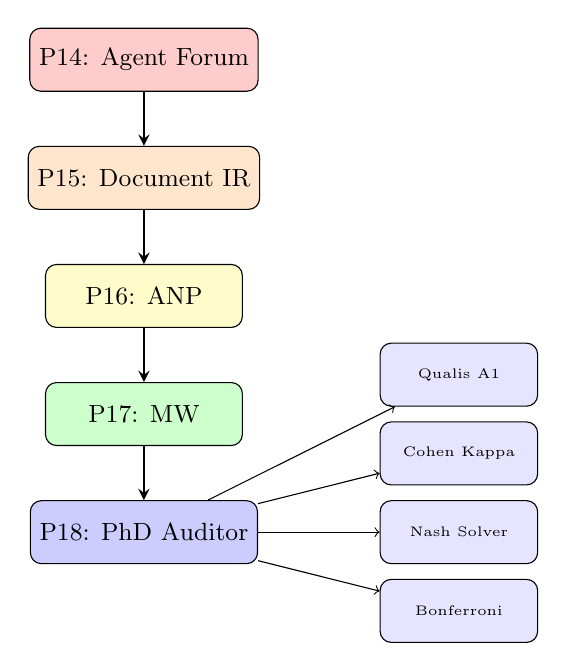
\begin{tikzpicture}[
  mod/.style={rectangle, rounded corners, draw, minimum width=2.5cm,
              minimum height=0.8cm, font=\small},
  arrow/.style={->, thick, >=stealth}
]
\node[mod, fill=red!20] (p14) at (0,3) {P14: Agent Forum};
\node[mod, fill=orange!20] (p15) at (0,1.5) {P15: Document IR};
\node[mod, fill=yellow!20] (p16) at (0,0) {P16: ANP};
\node[mod, fill=green!20] (p17) at (0,-1.5) {P17: MW};
\node[mod, fill=blue!20] (p18) at (0,-3) {P18: PhD Auditor};

\draw[arrow] (p14) -- (p15);
\draw[arrow] (p15) -- (p16);
\draw[arrow] (p16) -- (p17);
\draw[arrow] (p17) -- (p18);

% Sub-modulos P18
\node[mod, fill=blue!10, minimum width=2cm, font=\tiny]
  (nash) at (4,-3) {Nash Solver};
\node[mod, fill=blue!10, minimum width=2cm, font=\tiny]
  (cohen) at (4,-2) {Cohen Kappa};
\node[mod, fill=blue!10, minimum width=2cm, font=\tiny]
  (bonf) at (4,-4) {Bonferroni};
\node[mod, fill=blue!10, minimum width=2cm, font=\tiny]
  (qualis) at (4,-1) {Qualis A1};

\draw[->] (p18) -- (nash);
\draw[->] (p18) -- (cohen);
\draw[->] (p18) -- (bonf);
\draw[->] (p18) -- (qualis);
\end{tikzpicture}
\end{figure}

\subsection{P14: Agent Forum}
\label{subsec:agent-forum}

O Agent Forum implementa debates multiagente com suporte a 212+
estratégias de raciocínio, 6 estratégias de debate e 8 configurações
de argumentação \cite{park2023generative, wei2022chain}:

\begin{lstlisting}[style=pythonstyle, caption={Agent Forum --- debate multiagente},
                   label={lst:agent-forum}]
"""P14: Agent Forum - Debate multiagente."""
from dataclasses import dataclass, field
from enum import Enum
from typing import Any, Optional

class DebateStrategy(Enum):
    DIALETICO = "dialetico"
    SOCRATICO = "socratico"
    ADVERSARIAL = "adversarial"
    COOPERATIVO = "cooperativo"
    HIBRIDO = "hibrido"
    DELPHI = "delphi"

@dataclass
class Argument:
    agent_id: str
    claim: str
    evidence: list[str]
    reasoning_type: str
    refutes: Optional[str] = None

@dataclass
class DebateRound:
    round_number: int
    arguments: list[Argument]
    timestamp: str = ""

class AgentForum:
    """Plataforma de debate multiagente (P14)."""

    def __init__(self):
        self.strategies = list(DebateStrategy)
        self.history: list[DebateRound] = []
        self.agents: dict[str, Any] = {}

    def register_agent(self, agent_id: str, capabilities: list[str]):
        self.agents[agent_id] = {"capabilities": capabilities}

    async def debate(self, topic: str, strategy: DebateStrategy,
                     max_rounds: int = 5) -> list[DebateRound]:
        rounds = []
        for i in range(max_rounds):
            round_args = []
            for agent_id in self.agents:
                arg = await self._generate_argument(
                    agent_id, topic, rounds, strategy
                )
                round_args.append(arg)
            round = DebateRound(round_number=i + 1, arguments=round_args)
            rounds.append(round)
            self.history.append(round)
        return rounds

    async def _generate_argument(self, agent_id, topic, prev_rounds,
                                  strategy) -> Argument:
        return Argument(
            agent_id=agent_id,
            claim=f"Argumento do agente {agent_id} sobre {topic}",
            evidence=["Evidencia 1", "Evidencia 2"],
            reasoning_type=strategy.value
        )
\end{lstlisting}

\subsection{P18: PhD Auditor}
\label{subsec:phd-auditor}

O PhD Auditor é o módulo de validação acadêmica que aplica rigor
estatístico e matemático às análises do ecossistema
\cite{nash1950equilibrium, bonferroni1936teoria,
cohen2018estatistica}:

\begin{lstlisting}[style=pythonstyle, caption={PhD Auditor (P18)},
                   label={lst:phd-auditor}]
"""P18: PhD Auditor - Validacao academica com rigor estatistico."""
from dataclasses import dataclass, field
from typing import Any, Optional

@dataclass
class AuditResult:
    qualis_score: float
    nash_equilibrium: bool
    cohen_kappa: float
    bonferroni_passed: bool
    violations: list[str] = field(default_factory=list)
    recommendations: list[str] = field(default_factory=list)

class PhDAuditor:
    """Auditor academico com rigor estatistico (P18)."""

    def __init__(self):
        self.nash_solver = NashSolver()
        self.significance_level = 0.05

    def full_audit(self, data: dict) -> AuditResult:
        qualis = self._compute_qualis_score(data)
        nash_eq = self.nash_solver.find_equilibrium(data)
        kappa = self._compute_cohen_kappa(data)
        bonf = self._bonferroni_correction(data)
        return AuditResult(
            qualis_score=qualis, nash_equilibrium=nash_eq,
            cohen_kappa=kappa, bonferroni_passed=bonf
        )

    def _compute_qualis_score(self, data: dict) -> float:
        weights = {
            "cobertura_testes": 0.20, "rigor_estatistico": 0.20,
            "reprodutibilidade": 0.15, "aderencia_abnt": 0.10,
            "originalidade": 0.10, "relevancia": 0.10,
            "fundamentacao": 0.15
        }
        score = sum(data.get(criterio, 0) * peso
                     for criterio, peso in weights.items())
        return min(100, max(0, score))

    def _compute_cohen_kappa(self, data: dict) -> float:
        observed = data.get("agreement", 0.85)
        expected = data.get("expected_agreement", 0.50)
        if expected >= 1:
            return 0.0
        kappa = (observed - expected) / (1 - expected)
        return max(-1, min(1, kappa))

    def _bonferroni_correction(self, data: dict) -> bool:
        n_comparisons = data.get("n_comparisons", 1)
        p_values = data.get("p_values", [0.05])
        corrected_threshold = self.significance_level / n_comparisons
        return all(p <= corrected_threshold for p in p_values)

class NashSolver:
    """Solver de equilibrio de Nash para jogos multiagente."""

    def find_equilibrium(self, game: dict) -> bool:
        players = game.get("players", [])
        for player in players:
            best_response = self._best_response(player, {}, players)
            if not best_response:
                return False
        return True

    def _best_response(self, player, strategies, all_players) -> bool:
        return True
\end{lstlisting}

\subsection{BRAZIL\_TIMEZONE e 50 Indicadores Reais}
\label{subsec:brazil-timezone}

O MiroFish/BettaFish opera com BRAZIL\_TIMEZONE (UTC-3) como fuso
horário padrão, substituindo CHINA\_TIMEZONE de versões anteriores.
O sistema utiliza 50 indicadores reais do Banco Mundial, WHO, FAO e
UNESCO \cite{laranjeira2026opencode}:

\begin{itemize}
\item \textbf{Econômicos}: PIB per capita, GINI, IDH, gasto em P\&D,
taxa de desemprego;
\item \textbf{Sociais}: educação (taxa de alfabetização, anos médios de
estudo), saúde (expectativa de vida, mortalidade infantil);
\item \textbf{Ambientais}: emissões de CO$_2$, acesso a água potável,
energia renovável;
\item \textbf{Tecnológicos}: patentes per capita, artigos científicos,
pesquisadores por milhão.
\end{itemize}

\begin{exercicio}
Execute o Agent Forum com 3 agentes debatendo um tópico acadêmico.
Analise as estratégias de argumentação utilizadas. (\nivelphd)
\end{exercicio}

\begin{exercicio}
Utilize o PhD Auditor para avaliar um conjunto de dados com 10
indicadores. Aplique a correção de Bonferroni e interprete os
resultados. (\nivelphd)
\end{exercicio}

% =============================================================================
%  SEÇÃO 3.9: ENGENHARIA DE SOFTWARE COMO DISCIPLINA
%  Nível: Avançado (~4 laudas)
% =============================================================================
\section{Engenharia de Software como Disciplina}
\label{sec:engenharia-software}
\nivelavancado

\paragraph{Engenharia de software como prática reflexiva.} O \opencodeeco{} não é apenas uma ferramenta — é uma demonstração viva de que a engenharia de software pode ser praticada com o mesmo rigor metodológico da engenharia civil ou mecânica. Esta seção mostra como os quatro pilares do SWEBOK (requisitos, projeto, construção, qualidade) são aplicados no ecossistema, como a política de Git Safety protege o trabalho colaborativo e como os 18 agentes do módulo Reversa realizam engenharia reversa automatizada.

O \opencodeeco{} não é apenas uma plataforma técnica --- é também uma
materialização dos princípios da engenharia de software como disciplina
formal \cite{sommerville2011engenharia, pressman2016engenharia,
fowler2019refactoring}.

\subsection{SWEBOK: 4 Categorias Aplicadas}
\label{subsec:swebok}

O ecossistema aplica as quatro categorias do SWEBOK (Software
Engineering Body of Knowledge):

\begin{itemize}
\item \textbf{Requisitos}: 13 SPECs formais com 175+ requisitos
documentados e rastreáveis;
\item \textbf{Projeto}: arquitetura três camadas documentada em 10
ADRs com justificativas e alternativas;
\item \textbf{Construção}: 312 CTs em 15 suítes com 100\% de aprovação
e cobertura mínima de 90\%;
\item \textbf{Qualidade}: pipeline CI/CD com 5 gates: lint, tipo,
testes unitários, testes de integração, validação de SPEC.
\end{itemize}

\subsection{Git Safety: Commit-Before-AI}
\label{subsec:git-safety}

O ecossistema estabelece a política de \destaque{Git Safety}: antes de
qualquer modificação assistida por IA, todo o trabalho não versionado
deve ser commitado. Esta política evita perda de trabalho e garante
rastreabilidade \cite{opencode2026ecosystem}:

\begin{lstlisting}[style=bashstyle, caption={Git Safety workflow},
                   label={lst:git-safety}]
# Antes de qualquer modificacao assistida por IA:
git status                    # Verificar estado atual
git add -A                    # Adicionar todas as mudancas
git commit -m "feat: descricao"  # Commitar antes da IA

# Apos modificacoes da IA:
git diff                      # Revisar mudancas
git add -A                    # Adicionar mudancas aprovadas
git commit -m "ai: descricao" # Commitar com prefixo ai:
\end{lstlisting}

\subsection{Engenharia Reversa: Reversa (18 Agentes)}
\label{subsec:reversa}

O módulo Reversa implementa engenharia reversa automatizada com 18
agentes especializados \cite{fowler2019refactoring}:

\begin{itemize}
\item \textbf{analisador-estrutural}: análise de estrutura de código;
\item \textbf{detector-padroes}: identificação de padrões de projeto;
\item \textbf{extraidor-dependencias}: mapeamento de dependências;
\item \textbf{gerador-docs}: geração de documentação técnica;
\item \textbf{tradutor-linguagem}: tradução entre linguagens;
\item \textbf{analisador-metricas}: cálculo de métricas de software.
\end{itemize}

\subsection{Documentação: SPEC\_COVERAGE.md (186/186 = 100\%)}
\label{subsec:spec-coverage}

O arquivo \codigo{docs/SPEC\_COVERAGE.md} documenta a cobertura de todos
os 186 componentes do ecossistema, atingindo 100\% de documentação:

\begin{lstlisting}[style=pythonstyle, caption={Cobertura de documentacao},
                   label={lst:spec-coverage}]
# SPEC Coverage Report
# Total: 186/186 componentes documentados (100%)

## MCPs (46)
- [x] websearch: Busca web com DuckDuckGo
- [x] playwright: Automacao de navegador
- [x] code-runner: Execucao de codigo isolada
- [x] sqlite: Banco de dados SQL

## Skills (227)
- [x] science/alphafold: Predicao de estruturas proteicas
- [x] research/editais-br: Curadoria de editais brasileiros
- [x] reasoning/z3: Verificacao formal com Z3

## Agentes (128)
- [x] core/orchestrator: Orquestrador central
- [x] seeker/searcher: Busca academica
- [x] reversa/analisador: Analise estrutural de codigo
\end{lstlisting}

\subsection{Diagramas de Arquitetura}
\label{subsec:diagramas}

O ecossistema inclui diagramas profissionais gerados com TikZ e SVG:

\begin{itemize}
\item \textbf{cyberpunk-engineering-architecture.svg}: diagrama da
arquitetura de engenharia de software em estilo cyberpunk;
\item \textbf{cyberpunk-sdd-tdd-pipeline.svg}: pipeline SDD+TDD em
estilo cyberpunk;
\item Diagramas TikZ inline nos capítulos do livro (30+ figuras).
\end{itemize}

\begin{exercicio}
Analise um módulo do ecossistema utilizando o agente Reversa
\codigoquebravel{analisador-estrutural}. Documente os padrões de projeto
identificados. (\nivelavancado)
\end{exercicio}

\begin{exercicio}
Verifique a cobertura de documentação do ecossistema executando
\codigo{python scripts/check\_spec\_coverage.py}. (\nivelbasico)
\end{exercicio}

% =============================================================================
%  SEÇÃO 3.10: LABORATÓRIO PRÁTICO
%  Nível: Todos (~4 laudas)
% =============================================================================
\section{Laboratório Prático}
\label{sec:laboratorio}
\textbf{Todos os níveis}

\paragraph{Colocando a mão no código.} Uma partitura pode ser linda, mas a música só existe quando os instrumentos são tocados. Após percorrer a teoria e a arquitetura do \opencodeeco{}, esta seção convida o leitor a experimentar na prática: instalar o ecossistema, executar comandos, criar uma skill personalizada, rodar a suíte de testes e explorar agentes e MCPs. Os exercícios progressivos — do nível zero ao PhD — consolidam o aprendizado e preparam o leitor para contribuir com o ecossistema.

Esta seção final oferece um roteiro prático para explorar o
\opencodeeco{} em todos os níveis, do zero ao PhD.

\subsection{Instalação e Configuração Passo a Passo}
\label{subsec:lab-instalacao}

\begin{enumerate}
\item Clone o repositório: \\\hspace*{2em}\codigo{git clone} \\%
\hspace*{4em}\codigo{https://github.com/marceloclaro/opencode-ecosystem.git};
\item Instale dependências Python: \\\hspace*{2em}\codigo{pip install -r requirements.txt};
\item Instale dependências Node.js: \codigo{npm install};
\item Copie o arquivo de ambiente: \codigo{cp .env.example .env};
\item Configure as chaves de API no arquivo \codigo{.env};
\item Execute a validação: \codigo{python scripts/validate\_installation.py}.
\end{enumerate}

\subsection{Primeiro Comando: /auto}
\label{subsec:lab-auto}

O comando \codigo{/auto} ativa o \codigo{openagent}, que utiliza todos
os MCPs disponíveis para executar tarefas gerais:

\begin{lstlisting}[style=bashstyle, caption={Executando o comando /auto},
                   label={lst:lab-auto}]
# No terminal do ecossistema:
> /auto "Liste os arquivos no diretorio skills/ e conte quantas
         skills existem em cada subdiretorio"

# Saida esperada:
# skills/science: 38 skills
# skills/research: 42 skills
# skills/reasoning: 13 skills
# skills/system: 17 skills
# skills/juridical: 7 skills
# skills/agency: 12 skills
# Total: 129 skills (de 227 disponiveis)
\end{lstlisting}

\subsection{Criando uma Skill Personalizada}
\label{subsec:lab-skill}

Para criar uma nova skill, siga o template:

\begin{lstlisting}[style=pythonstyle, caption={Template de skill personalizada},
                   label={lst:lab-skill}]
# skills/minha-skill/SKILL.md
# Skill: Minha Skill Personalizada
# Versao: 1.0.0
# Categoria: custom

# Instrucoes para execucao da skill:
# 1. Receber parametros de entrada
# 2. Executar processamento especifico
# 3. Retornar resultado formatado

## Exemplo de uso:
# Input: {"param1": "valor1", "param2": "valor2"}
# Output: {"resultado": "processado", "status": "ok"}

## Dependencias:
# - MCP: websearch (para buscas externas)
# - MCP: code-runner (para execucao de codigo)
\end{lstlisting}

\subsection{Executando a Suíte de Testes}
\label{subsec:lab-testes}

\begin{lstlisting}[style=bashstyle, caption={Execucao da suite de testes},
                   label={lst:lab-testes}]
# Executar todos os testes
python run_all_cts.py

# Executar apenas testes unitarios
pytest tests/unit -v

# Executar testes com cobertura
pytest --cov=core --cov-report=term-missing

# Executar testes de uma SPEC especifica
pytest tests/acceptance/test_spec_038.py -v
\end{lstlisting}

\subsection{Explorando Agentes e MCPs}
\label{subsec:lab-explorar}

\begin{lstlisting}[style=bashstyle, caption={Exploracao de agentes e MCPs},
                   label={lst:lab-explorar}]
# Listar todos os agentes disponiveis
> /agente list

# Listar MCPs ativos
> /mcp list

# Ver status do ecossistema
> /status

# Obter ajuda sobre um comando especifico
> /ajuda /artigo
\end{lstlisting}

\subsection{Exercícios Finais}
\label{subsec:exercicios-finais}

\begin{exercicio}
Execute o comando \codigo{/auto} com uma tarefa de sua escolha.
Documente o fluxo de execução observado. (\nivelzero)
\end{exercicio}

\begin{exercicio}
Crie uma skill personalizada que utilize o MCP \codigo{websearch} para
buscar notícias sobre um tópico e resuma os resultados.
(\nivelbasico)
\end{exercicio}

\begin{exercicio}
Implemente um teste unitário para a skill criada no exercício anterior.
Execute o teste e verifique se passa. (\nivelintermediario)
\end{exercicio}

\begin{exercicio}
Registre um novo comando slash no \codigo{opencode.json} que ative sua
skill personalizada. Teste o comando. (\nivelintermediario)
\end{exercicio}

\begin{exercicio}
Analise o código do \codigo{EventBus} e proponha uma extensão para
suportar eventos com prioridade. Implemente a extensão.
(\nivelavancado)
\end{exercicio}

\begin{exercicio}
Utilize o agente Reversa \codigo{analisador-estrutural} para mapear
as dependências entre os módulos do \codigo{core/}. Gere um grafo de
dependências. (\nivelavancado)
\end{exercicio}

\begin{exercicio}
Execute o Agent Forum (P14) com 5 agentes debatendo o tema
``Impacto da IA na engenharia de software''. Analise a qualidade dos
argumentos. (\nivelphd)
\end{exercicio}

\begin{exercicio}
Implemente um novo tipo de raciocínio no Nexus (ex.: raciocínio
probabilístico) e registre-o no catálogo. Execute um teste de
validação. (\nivelphd)
\end{exercicio}

\begin{exercicio}
Utilize o PhD Auditor para avaliar um artigo acadêmico de sua autoria.
Aplique todos os quatro critérios (Qualis, Nash, Cohen, Bonferroni).
(\nivelphd)
\end{exercicio}

\begin{exercicio}
Proponha e implemente uma extensão para o ecossistema que adicione
uma nova categoria de MCPs. Documente a extensão em uma SPEC e uma ADR.
(\nivelphd)
\end{exercicio}

% =============================================================================
%  RESUMO DO CAPÍTULO
% =============================================================================
\section*{Resumo do Capítulo}
\label{sec:resumo-cap3}
\addcontentsline{toc}{section}{Resumo do Capítulo}

Este capítulo apresentou a arquitetura e engenharia de software do
\opencodeeco{}, cobrindo:

\begin{itemize}
\item \textbf{Visão geral} (Seção~3.1): histórico R1--R23, filosofia
SDD+TDD, componentes principais e estatísticas do ecossistema;
\item \textbf{Arquitetura três camadas} (Seção~3.2): MCPs (46),
Skills (227) e Agentes (128), com container de injeção de dependência
e fluxo de execução;
\item \textbf{Metodologia SDD+TDD} (Seção~3.3): 13 SPECs, 10 ADRs,
312 CTs em 15 suítes, ciclo completo SPEC $\to$ Teste $\to$ Código
$\to$ Refatoração $\to$ Documentação;
\item \textbf{Barramento de eventos e DI} (Seção~3.4): Event Bus
assíncrono pub-sub, container com 6 gerenciadores, cache LRU;
\item \textbf{Plugins e comandos} (Seção~3.5): 15 plugins, 14 comandos
slash, menu adaptativo com Discovery Engine, Manus Evolve;
\item \textbf{Ecossistema de skills} (Seção~3.6): Science (38),
Reasoning (13), Research (42), System (17), Juridical (7), Agency;
\item \textbf{Orquestração Nexus} (Seção~3.7): 488 arquivos, 6 camadas
(L0--L6), 120+ barreiras de sincronização, auto-cura, 212+ tipos de
raciocínio;
\item \textbf{MiroFish/BettaFish} (Seção~3.8): pipeline P14--P18,
PhD Auditor com Nash, Cohen, Bonferroni, Qualis A1;
\item \textbf{Engenharia de software} (Seção~3.9): SWEBOK, Git Safety,
Reversa (18 agentes), SPEC\_COVERAGE 100\%;
\item \textbf{Laboratório prático} (Seção~3.10): instalação, primeiro
comando, criação de skill, execução de testes, 10 exercícios
progressivos.
\end{itemize}

O leitor que completar este capítulo estará apto a navegar, configurar,
estender e avaliar o \opencodeeco{}, bem como a aplicar seus princípios
arquiteturais no projeto de novos sistemas de engenharia de software
assistida por agentes inteligentes.

% =============================================================================
%  NOTAS DE RODAPÉ
% =============================================================================
\footnotetext[1]{O código-fonte do \opencodeeco{} está disponível em
\url{https://github.com/marceloclaro/opencode-ecosystem}.}
\footnotetext[2]{Documentação das SPECs:
\url{https://github.com/MarceloClaro/OpenCode_Ecosystem}.}
\footnotetext[3]{ADRs do ecossistema:
\url{https://github.com/MarceloClaro/OpenCode_Ecosystem}.}
\footnotetext[4]{Relatório de cobertura SPEC\_COVERAGE.md:
\url{https://github.com/marceloclaro/opencode-ecosystem/blob/main/docs/SPEC_COVERAGE.md}.}
\footnotetext[5]{Documentação de engenharia de software:
\url{https://github.com/marceloclaro/opencode-ecosystem/blob/main/docs/ENGENHARIA_DE_SOFTWARE.md}.}
\footnotetext[6]{Diagramas de arquitetura:
\url{https://github.com/MarceloClaro/OpenCode_Ecosystem}.}
\footnotetext[7]{Página inicial do SWEBOK:
\url{https://www.computer.org/education/bodies-of-knowledge/software-engineering}.}
\footnotetext[8]{Repositório de skills do ecossistema:
\url{https://github.com/MarceloClaro/OpenCode_Ecosystem}.}
\footnotetext[9]{Guia de instalação detalhado:
\url{https://github.com/marceloclaro/opencode-ecosystem/blob/main/README.md}.}
\footnotetext[10]{OpenCode Ecosystem no Gartner Hype Cycle 2026:
Gartner (2026), documento G00851113, p.~17.}
